\documentclass[10pt, ucs, notheorems, handout]{beamer}

\usetheme[numbers,totalnumbers,minimal]{Statmod}
\usefonttheme[onlymath]{serif}
\setbeamertemplate{navigation symbols}{}
\setbeamercolor{alerted text}{fg=blue}

\mode<handout> {
    \usepackage{pgfpages}
    \setbeameroption{show notes}
    \pgfpagesuselayout{2 on 1}[a4paper, border shrink=5mm]
}

\usepackage[utf8x]{inputenc}
\usepackage[T2A]{fontenc}
\usepackage[russian]{babel}
\usepackage{tikz}
\usepackage{ragged2e}
\usepackage{xcolor}
\usepackage{bm}

\newcommand{\tX}[1]{\mathsf{#1}}
\DeclareMathOperator*{\argminB}{argmin}   % Jan Hlavacek
\DeclareMathOperator{\diag}{diag}
\newcommand{\norm}[1]{\left\lVert#1\right\rVert}
\newcommand{\E}{\mbox{E}}
\newcommand{\D}{\mbox{D}}

\newtheorem{theorem}{Утверждение}
\newtheorem{example}{Пример}
\newtheorem{definition}{Определение}
\newtheorem{task}{Задача}
\newtheorem{def1}{Определение}
\newtheorem{proposition}{Утверждение}
\newtheorem{notice}{Замечание}



\title[Робастные варианты метода SSA]{%
    Робастные варианты метода анализа сингулярного спектра}

\author{Третьякова Александра Леонидовна}

%\institute[Санкт-Петербургский Государственный Университет]{%
%    \small
%    Санкт-Петербургский государственный университет\\
%    Прикладная математика и информатика\\
%    Вычислительная стохастика и статистические модели\\
%    \vspace{1.25cm}
%    Преддипломная практика}

\institute[СПбГУ]{Санкт-Петербургский государственный университет \\
	Математико-механический факультет \\
	Кафедра статистического моделирования \\
	\vspace{0.4cm}
	Научный руководитель: к.ф.-м.н., доц. Голяндина Н.Э. \\
	Рецензент: к.ф.-м.н. Пепелышев А.Н.
	\vspace{0.3cm}
}

\date[Защита]{Санкт-Петербург, 2020}

\subject{Talks}

\begin{document}

\begin{frame}[plain]
    \titlepage

    \note{Выпускная работа посвящена разработке и исследованию модификаций метода анализа сингулярного спектра, устойчивых к выбросам. \\
    Работа выполнена на кафедре статистического моделирования,\\
    руководитель к.ф.-м.н., доц. Голяндина Н.Э.}
\end{frame}



\setbeameroption{show notes}

\begin{frame}
\frametitle{Постановка задачи}
Рассмотрим вещественнозначный \alert{временной ряд} $\tX{X}=(x_1, \ldots, x_{N})$, где $N$~--- длина ряда.\\

Предполагаем, что $x_i = s_i + r_i$, $i=1,\ldots,N$, где $r_i$ --- шум.
\begin{task}
	Разложение временного ряда на интерпретируемые аддитивные составляющие: \\
	\begin{equation*}
	\tX{X}=\tX{S}+\tX{R},
	\end{equation*}
	$\tX{S}$~--- \alert{сигнал,}\\
	$\tX{R}$~--- \alert{шум.}\\
\end{task}
\alert{Метод:} <<Гусеница>>-SSA (Singular Spectrum Analysis) [Analysis of Time Series
Structure: SSA and Related Techniques, Golyandina N., Nekrutkin V.,
Zhigljavsky A., 2001].

\note{
В реальной жизни часто возникают задачи исследования различных процессов с течением времени.
%Пусть имеется $x(t)$ --- функция, описывающая некоторый процесс во времени. Если произвести измерения через одинаковые промежутки времени $t_i$, где $i=1,\ldots,N$, тогда $x_i=x(t_i)$ представляют собой временной ряд $\tX{X}=(x_1,\ldots,x_N)$. \\
Работа посвящена одному из методов исследования временных рядов --- методу анализа сингулярного спектра (Singular Spectrum Analysis, SSA), который позволяет анализировать ряд без задания его параметрической модели. Пусть имеется временной ряд $\tX{X}$ длины 𝑁, который представляет собой сумму сигнала и шума. Данный метод позволяет получить разложение интересующего нас временного ряда $\tX{X}$ на интерпретируемые аддитивные составляющие: $\tX{X} = \tX{S} + \tX{R}$, где $\tX{S}$~---~сигнал, $\tX{R}$ --- шум.
}
\end{frame}

\begin{frame}
\frametitle{Постановка задачи}
\begin{figure}[h]
	\begin{minipage}[h]{0.49\linewidth}
		\center{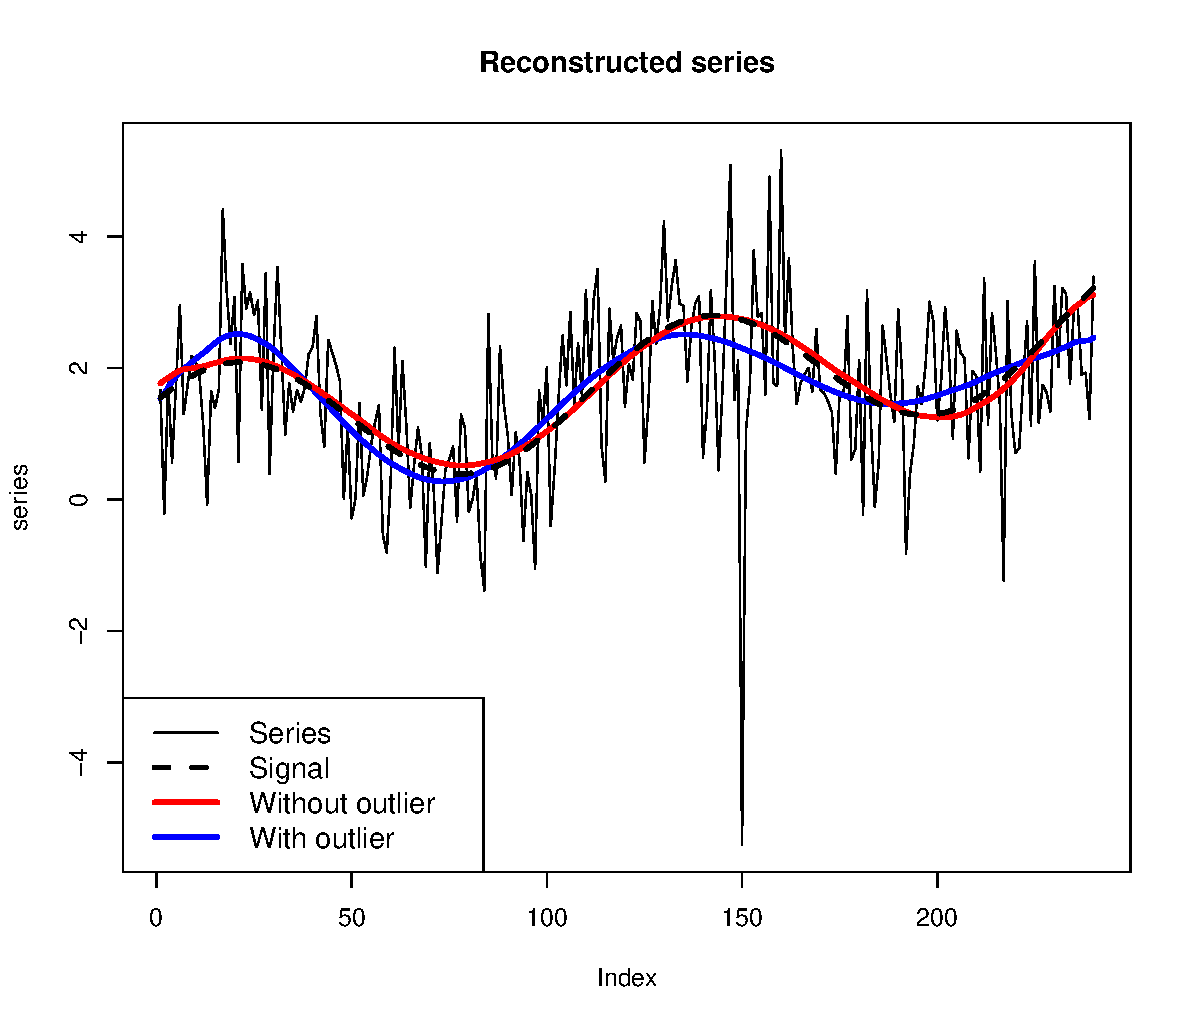
\includegraphics[width=1.09\linewidth]{RecSeries} \\ }
	\end{minipage}
	\hfill
	\begin{minipage}[h]{0.49\linewidth}
		\center{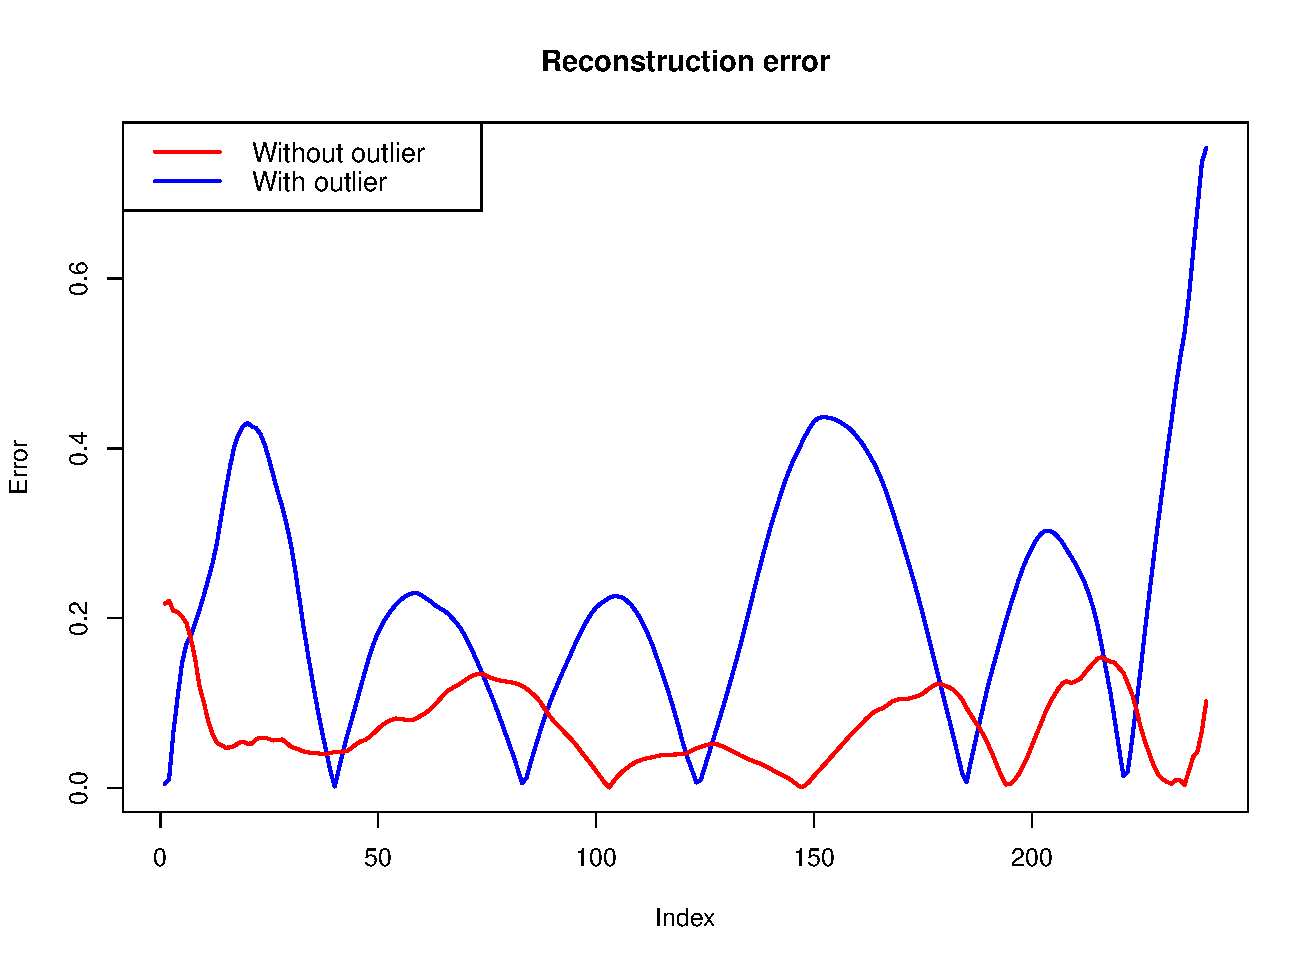
\includegraphics[width=1.09\linewidth]{RecErrorAbs} \\}
	\end{minipage}
	\caption{График ряда с выделяющимся наблюдением и модуль ошибок восстановления сигнала в присутствии выброса и без него.}
	\label{ris:image1}
\end{figure}
\alert{Задача:} предложить устойчивые к выбросам модификации метода анализа сингулярного спектра и сравнить их между собой.

\note{
	Однако на практике часто возникают выделяющиеся наблюдения или выбросы. Это могут быть ошибки в данных или сбои в работе измерительного прибора, которые могут сильно повлиять на
	восстановление сигнала методом SSA. На рисунках представлен график ряда с выбросом и восстановление сигнала в присутствии выделяющегося наблюдения (синяя линяя) и без него (красная линия), а также модуль ошибки выделения сигнала. Видно, что выброс сильно портит восстановление сигнала.
	Поэтому значительный интерес представляет разработка устойчивых к выбросам модификаций метода SSA и сравнение их между собой, а также с классическим методом SSA.
}
\end{frame}

\begin{frame}
\frametitle{Постановка задачи}
Задачи:
\begin{itemize}
	\item Обзор и структурирование устойчивых вариантов метода SSA,
	\item Предложение модификации для нестационарного шума,
	\item Сравнение рассмотренных методов по трудоемкости,
	\item Сравнение рассмотренных методов по точности на примерах.
\end{itemize}

\note{
	Задачами работы являются обзор и структурирование устойчивых вариантов метода SSA, предложение модификации для нестационарного шума, а также сравнение рассмотренных методов по трудоемкости и точности на различных примерах.
}
\end{frame}

\begin{frame}
\frametitle{Метод SSA для выделения сигнала ранга, не превосходящего $r$}
Ряд $\tX{X}=(x_1, \ldots, x_{N})$.

Пусть $0<L<N$~--- длина окна. $K=N-L+1$. 

Обозначим  $\mathcal{M}$ --- пространство матриц $L\times K$,

$\mathcal{M}_{\mathcal{H}}$ --- пространство ганкелевых матриц $L\times K$,

$\mathcal{M}_{r}$ --- множество матриц ранга, не превосходящего $r$. \\
~~\\

Ряд $\mapsto$ \alert{траекторная матрица}  $\mathbf{X}$: \\
~~\\

$\mathbf{X}=[X_1:\ldots:X_K]
=\left( \begin{array} {ccccc}
x_1 & x_2 & x_3&\ldots &x_{K}  \\
x_2 & x_3 & x_4&\ldots &x_{K+1} \\
x_3 & x_4 & x_5&\ldots &x_{K+2} \\
\vdots& \vdots& \vdots&\ddots &\vdots  \\
x_{L}& x_{L+1} & x_{L+2}&\ldots &x_{N}  \\
\end{array}\right)$. 
\note{
	 Для начала опишем алгоритм метода SSA для выделения сигнала ранга, не превосходящего r.
	 
	  Пусть имеется ряд длины $N$. Выберем целое число $L$ --- длина окна, $K$ полагаем равным $N-L+1$. Введем пространство ганкелевых матриц (матрица называется ганкелевой, если ее элементы на антидиагоналях равны между собой), а также множество матриц ранга, не превосходящего $r$. Введем понятие траекторной матрицы, состоящей из векторов вложения $(x_1,\ldots,x_L)^\mathrm{T},$ $(x_2,\ldots,x_{L+1})^\mathrm{T}$ и так далее.
}
\end{frame}

\begin{frame}
\begin{itemize} 
\item{ Оператор вложения $\mathcal{T}:\mathbb{R}^N \rightarrow \mathcal{M}_{\mathcal{H}}: \mathcal{T} (\tX{X}) = \mathbf{X} $.
}
\item{ $\Pi_{r}:\mathcal{M}\rightarrow \mathcal{M}_r$ --- проектор на множество матриц ранга, не превосходящего $r$.
}
\item{
	$\Pi_{\mathcal{H}}:\mathcal{M} \rightarrow \mathcal{M}_{\mathcal{H}}$ --- проектор на пространство ганкелевых матриц.
}
\end{itemize}

Структура сигнала $\tX{S}$: ранг траекторной (ганкелевой) матрицы $\mathcal{T} (\tX{S})$ равен $r$. \\
~~\\

В результате получаем оценку сигнала:
\begin{equation*}
\tilde{\tX{S}} = \mathcal{T}^{-1} \Pi_{\mathcal{H}} \Pi_{r} \mathcal{T} (\tX{X}), 
\end{equation*}
где проекторы можно строить по различным нормам. \\
~~\\
Будем рассматривать следующие варианты: 
\begin{itemize}
	\item Проекторы $\Pi_r$ и $\Pi_{\mathcal{H}}$ по норме в $\mathbb{L}_2$ (стандартный L2-SSA),
	\item Проекторы $\Pi_r$ и $\Pi_{\mathcal{H}}$ по норме в $\mathbb{L}_1$ (L1-SSA),
	\item Проекторы $\Pi_r$ и $\Pi_{\mathcal{H}}$ по взвешенной норме в $\mathbb{L}_2$ (WL2-SSA).
\end{itemize}
\note{
	Введем оператор вложения $\mathcal{T}$, который переводит ряд в траекторную матрицу. А также два проектора: $\Pi_{r}$ --- проектор на множество матриц ранга, не превосходящего $r$, и $\Pi_{\mathcal{H}}$ --- проектор на пространство ганкелевых матриц. Предполагаем, что ранг траекторной матрицы сигнала  равен $r$.  Для того, чтобы получить оценку сигнала, необходимо сначала применить оператор вложения, получить из ряда траекторную матрицу. Затем сделать проекцию на множество матриц ранга, не превосходящего $r$, затем проекцию на пространство ганкелевых матриц, и снова превратить в ряд. \\ 
	Проекторы можно строить по различным нормам. Для построения устойчивых модификаций рассмотрим два подхода. Первый подход состоит в использовании нормы в пространстве $\mathbb{L}_1$, которая является более устойчивой к выбросам. Второй подход --- использование взвешенной нормы в $\mathbb{L}_2$, где точкам, содержащим выбросы, присваивается меньший вес. Таким образом, будем рассматривать следующие варианты: обычный SSA, где проекторы строятся по нормам в пространстве $\mathbb{L}_2$, вариант с проекторами по норме в пространстве $\mathbb{L}_1$ и вариант с проекторами по взвешенной норме в $\mathbb{L}_2$.
}
\end{frame}

\begin{frame}
\frametitle{L2-SSA. Вид проекторов по норме в $\mathbb{L}_2$}
\begin{def1} 
Пусть $\mathbf{A}$ --- матрица $L\times K$.

Норма в пространстве $\mathbb{L}_2$ (норма Фробениуса):  $\|\mathbf{A}\|_\mathrm{F} = \sqrt{\sum\limits_{i=1}^{L} {\sum\limits_{j=1}^{K} a_{ij}^2}}$.			
\end{def1}
\begin{itemize}
\item
$\Pi_{\mathcal{H}}$ --- проектор на множество ганкелевых матриц по норме Фробениуса посредством усреднения элементов на диагоналях $i+j=\text{const}$:
$\|\mathbf{X}-\mathbf{Y}\|_\mathrm{F}^2 \longrightarrow \min\limits_{Y \in \mathcal{M}_{\mathcal{H}} } $.\\
\item
$\Pi_{r}$ --- проектор на множество матриц ранга $r$ по норме Фробениуса:  $\|\mathbf{X}-\mathbf{Y}\|_\mathrm{F}^2 \longrightarrow \min\limits_{Y \in \mathcal{M}_{r} } $, $\mathbf{Y}=\sum \limits_{i=1}^{r}{\sqrt{\lambda_i}U_iV_i^\mathrm{T}}$.
\end{itemize}
\note{
	Опишем, как строятся проекторы по норме в пространстве $\mathbb{L}_2$ (норма Фробениуса). Проектор на множество ганкелевых матриц строится посредством усреднения элементов на побочных диагоналях. 
	
	Для того, чтобы получить проекцию на множество матриц ранга, не превосходящего $r$, необходимо взять первые $r$ компонент сингулярного разложения траекторной матрицы ряда.
}
\end{frame}

\begin{frame}
\frametitle{L1-SSA. Вид проекторов по норме в $\mathbb{L}_1$}
\begin{def1} 
Пусть $\mathbf{A}$ --- матрица $L\times K$.

Норма в пространстве $\mathbb{L}_1$ :  $\|\mathbf{A}\|_1 = \sum\limits_{i,j}^{} {|a_{ij}|}$.		
\end{def1}
\begin{notice}
Так как	$\argminB\limits_a \mathbb{E} |\xi - a| = \mathrm{med} \xi $, то $\Pi_{\mathcal{H}}$ строится посредством выбора медианы значений на диагоналях $i+j=\text{const}$.
\end{notice}
Для построения проектора на множество матриц ранга $r$ в $\mathbb{L}_1$ будем рассматривать \alert{последовательный метод}.
\note{
	Для получения проекции на множество ганкелевых матриц по норме в пространстве $\mathbb{L}_1$, необходимо взять медиану значений на побочных диагоналях. Однако решения в явном виде задачи построения проектора на множество матриц ранга, не превосходящего $r$, в пространстве $\mathbb{L}_1$ нет. Мы будем рассматривать последовательный метод для решения этой задачи, который находит решение задачи итеративно.
}
\end{frame}

\begin{frame}
\frametitle{L1-SSA. Реализация. Последовательный метод}
\small{
В R-пакете pcaL1 [Jot et al., 2017] имеется реализация последовательного метода решения задачи $\|\mathbf{Y}-\mathbf{U}\mathbf{V}^{\mathrm{T}}\|_1 \longrightarrow \min\limits_{\mathbf{U},\mathbf{V}}.$ }%~~ \mathbf{U}^{\mathrm{T}}\mathbf{U} = \mathbf{I}_r$.

\alert{Алгоритм l1pca} [Brooks J. P., Jot S., 2013] :\\
\small{
\begin{enumerate}
\item Инициализация $\mathbf{U}(0)\in \mathbb{R}^{L\times r}$, нормировка столбцов  $\mathbf{U}(0)$,
\item $t:=t+1$,
\item  $\mathbf{V}(t) = \argminB\limits_{\mathbf{V}\in \mathbb{R}^{K\times r}} \|\mathbf{Y}-\mathbf{U}(t-1)\mathbf{V}^{\mathrm{T}}\|_1$ 

\footnotesize{Задача разбивается на $K$ независимых подзадач вида $\mathbf{v}_i = \argminB\limits_{\mathbf{x}} \|Y_i-\mathbf{U}(t-1)\mathbf{x}\|_1$,
где $Y_i\in \mathbb{R}^L$ --- столбцы $\mathbf{Y}$, $\mathbf{v}_i\in\mathbb{R}^r$ --- строки $\mathbf{V}$, $i=1,\ldots,K$},
\small{
\item  $\mathbf{U}(t) = \argminB\limits_{\mathbf{U}\in \mathbb{R}^{L\times r}} \|\mathbf{Y}-\mathbf{U}\mathbf{V}^{\mathrm{T}}(t)\|_1$ (решается аналогично п.3)
\item Нормировка столбцов $\mathbf{U}(t)$,
\item  if $\mathbf{U}(t) \ne \mathbf{U}(t-1)$ (по крит. остановки) then Go to Step 2 \\
else $\mathbf{U}:=\mathbf{U}(t);~ \mathbf{V}:=\mathbf{V}(t)$.
}
\end{enumerate}
}
\small{
Крит. остановки: $\max \limits_{i=1,\ldots,L, j=1,\ldots,r} |u_{ij}(t) - u_{ij}(t-1)| > \varepsilon$ или $t>N_{\text{iter}}$.}

\normalsize{Решаем задачу, меняя на каждой итерации $\mathbf{U}$ и $\mathbf{V}$ и разбивая исходную задачу на линейные подзадачи.}
\note{
	Сам алгоритм описан в статье 2013 года, в R-пакете pcaL1 имеется его реализация. Задача представляется в виде $\|\mathbf{Y}-\mathbf{U}\mathbf{V}^{\mathrm{T}}\|_1 \longrightarrow 
	\min\limits_{\mathbf{U},\mathbf{V}}$.  Алгоритм итеративный, на каждой итерации фиксируем $\mathbf{U}$ и решаем задачу относительно $\mathbf{V}$. Затем фиксируем $\mathbf{V}$ и минимизируем по $\mathbf{U}$, пока не выполнен критерий остановки. %Каждая из подзадач сводится к решению задач линейного программирования с ограничениями.
	
	Задачу из пункта 3 алгоритма можно разбить на $K$ независимых подзадач. С помощью решения каждой такой подзадачи получаем оценку $\mathbf{v}_i$, $i=1,\ldots,K$ --- строк матрицы $\mathbf{V}$. Согласно [Ke Q., Kanade T., 2005], каждая подзадача сводится к задаче линейного программирования с ограничениями. %Задача линейного программирования находит минимальную границу $\bm{\delta}$ такую, что область $$ -\bm{\delta} \le Y_i - \mathbf{U}(t-1)\mathbf{x} \le \bm{\delta}$$  является непустой.
	Задача из пункта 4 алгоритма решается аналогичным образом.
	
	Таким образом, мы решаем задачу, фиксируя и меняя на каждой итерации $\mathbf{U}$ и $\mathbf{V}$, разбивая исходную задачу на линейные подзадачи.
}
\end{frame}

%\begin{frame}
%\frametitle{L1-SSA. Реализация. Последовательный метод}
%Задача $\mathbf{V}(t) = \argminB\limits_{\mathbf{V}\in \mathbb{R}^{K\times r}} \|\mathbf{Y}-\mathbf{U}(t-1)\mathbf{V}^{\mathrm{T}}\|_1$ (пункты 3 и 4 алгоритма) может быть разбита на $K$ независимых небольших подзадач 
%\begin{equation}\label{subtask}
%\mathbf{v}_i = \argminB\limits_{\mathbf{x}} \|Y_i-\mathbf{U}(t-1)\mathbf{x}\|_1,
%\end{equation}
% где $Y_i\in \mathbb{R}^L$ --- столбцы $\mathbf{Y}$, $\mathbf{v}_i\in\mathbb{R}^r$ --- строки $\mathbf{V}$, $i=1,\ldots,K$.
% Глобальное решение задачи~(\ref{subtask}) находится с помощью задачи линейного программирования  
%\begin{equation*}
%\min_{\bm{\delta}} \mathbf{1}^\mathrm{T}\bm{\delta}
%\end{equation*}
%с ограничениями $$ -\bm{\delta} \le Y_i - \mathbf{U}(t-1)\mathbf{x} \le \bm{\delta},$$ где $\mathbf{1} \in \mathbb{R}^L$ --- вектор-столбец, состоящий из единиц ([Ke Q., Kanade~T., 2005]). 
%
%\note{
%	Задачу из пункта 3 алгоритма можно разбить на $K$ независимых подзадач. С помощью решения каждой такой подзадачи получаем оценку $\mathbf{v}_i$, $i=1,\ldots,K$ --- строк матрицы $\mathbf{V}$. Согласно [Ke Q., Kanade T., 2005], решение каждой подзадачи находится с помощью задачи линейного программирования, представленной на слайде. %Задача линейного программирования находит минимальную границу $\bm{\delta}$ такую, что область $$ -\bm{\delta} \le Y_i - \mathbf{U}(t-1)\mathbf{x} \le \bm{\delta}$$  является непустой.
%	
%	Задача из пункта 4 алгоритма решается аналогичным образом.
%}
%
%\end{frame}


\begin{frame}
\frametitle{WL2-SSA. Вид проекторов по взвешенной норме в $\mathbb{L}_2$}
\begin{def1} 
Пусть $\mathbf{A}$ --- матрица $L\times K$, $\mathbf{W}$ --- матрица весов $L\times K$.

Норма в пространстве $\mathbb{L}_2$ с весами $\mathbf{W}$:  $\|\mathbf{A}\|_\mathrm{W} = \sqrt{\sum\limits_{i=1}^{L} {\sum\limits_{j=1}^{K} w_{ij} a_{ij}^2}}$.			
\end{def1}
\begin{proposition}[Zvonarev, Golyandina, 2015]
Для построения проекции $\Pi_{\mathcal{H}}\mathbf{Y} = \widehat{\mathbf{Y}} = \{\widehat{y}_{ij}\}_{i,j = 1}^{L,K}$  необходимо суммировать элементы на диагоналях $i+j=\text{const}$ с весами и нормировать на сумму весов: $\widehat{y}_{ij} = \frac{\sum\limits_{l,k: l+k=i+j} w_{lk}y_{lk}}{\sum\limits_{l,k: l+k=i+j} w_{lk}}$.
\end{proposition}
\alert{Замечание}: 	В случае ганкелевой матрицы весов $\mathbf{W}$ проектор на пространство ганкелевых матриц по взвешенной норме в $\mathbb{L}_2$ совпадает с проектором на пространство ганкелевых матриц по норме в  $\mathbb{L}_2$.
\note{
	Введем норму в пространстве $\mathbb{L}_2$ с весами $\mathbf{W}$. Для построения проекции на пространство ганкелевых матриц необходимо суммировать элементы на побочных диагоналях с весами и нормировать на сумму весов. 
	Можно заметить, что если матрица весов ганкелева, то проектор на пространство ганкелевых матриц по взвешенной норме в $\mathbb{L}_2$ совпадает с проектором на пространство ганкелевых матриц по норме в  $\mathbb{L}_2$.
	
	Далее рассмотрим построение проектора по взвешенной норме в $\mathbb{L}_2$ на множество матриц ранга, не превосходящего $r$.
}

\end{frame}




\begin{frame}
\frametitle{WL2-SSA. Метод с итеративным обновлением весов}
\small
Пусть $\mathbf{Y} \in \mathbb{R}^{L\times K}$ --- траекторная матрица ряда,  $\widehat{\mathbf{Y}} = \mathbf{U}\mathbf{V}^{\mathrm{T}} = \{\widehat{y}_{ij}\}_{i,j=1}^{L,K}$.
Решаем задачу
\begin{equation*}
\norm{\mathbf{W}^{1/2}\odot(\mathbf{Y}-\mathbf{U}\mathbf{V}^{\mathrm{T}})}^2_F \longrightarrow \min_{\mathbf{U},\mathbf{V}}, 
\end{equation*}
%\footnotesize Рассмотрим задачу 
%\begin{equation*}
% \|\mathbf{Y}-\hat{\mathbf{Y}}\|_\rho = \|\mathbf{Y}-\mathbf{U}\mathbf{V}^{\textrm{T}}\|_\rho = \sum_{i=1}^L \sum_{j=1}^K \rho_\alpha (\frac{y_{ij}-\hat{y}_{ij}}{\sigma})  \longrightarrow \min_{\hat{\mathbf{Y}} \in \mathcal{M}_r},
%\end{equation*}	
%где  $\rho_\alpha (x) = 
%\begin{cases}
%\frac{1}{6}\alpha^2\{1-(1-(\frac{|x|}{\alpha})^2)^3\}, &|x|\le\alpha\\
%\frac{1}{6}\alpha^2, &|x|>\alpha
%\end{cases}$ --- функция Тьюки.

где $\odot$ --- поэлементное умножение, $\mathbf{W}^{1/2}$ --- поэлементное взятие корня, веса $w_{ij} = w(\frac{y_{ij}-\hat{y}_{ij}}{\sigma_{ij}})$ вычисляются по формуле %$w(x)=\frac{\partial \rho(x)}{\partial |x|} \frac{1}{|x|}$:~~~ 
$w(x) = 
\begin{cases}
(1-(\frac{|x|}{\alpha})^2)^2, &|x|\le\alpha\\
0, &|x|>\alpha
\end{cases}.$

Значения $\alpha$ и $\{\sigma_{ij},~ i=1,\ldots,L,~j=1,\ldots,K\}$ --- параметры.
\begin{figure}[!h]
\center{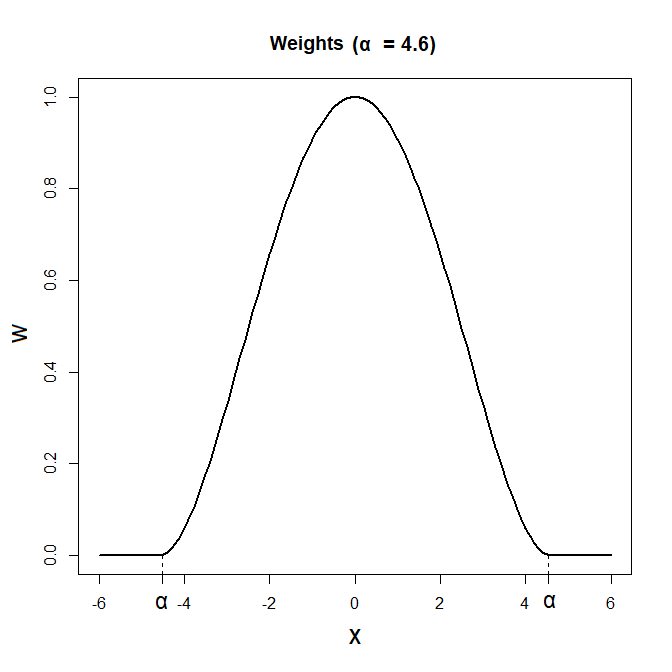
\includegraphics[width=0.33\linewidth]{weights1}}
\caption{График функции $w(x)$.}
\label{Tukey}
\end{figure}

\note{
Пусть $\mathbf{Y} \in \mathbb{R}^{L\times K}$ --- траекторная матрица ряда. Решаем задачу $\norm{\mathbf{W}^{1/2}\odot(\mathbf{Y}-\mathbf{U}\mathbf{V}^{\mathrm{T}})}^2_F \longrightarrow \min\limits_{\mathbf{U},\mathbf{V}}$, где веса вычисляются по определенной формуле, как в известном методе локальной регрессии loess. Имеются параметры $\alpha$ и $\sigma_{ij}$. Их выбор мы обсудим далее. График весовой функции $w(x)$ представлен на слайде. Значение веса зависит от нормированных остатков: если остаток маленький по модулю, то вес максимальный, если остаток по модулю превосходит заданный параметр $\alpha$, то вес обнуляется. 
}
\end{frame}

\begin{frame}
\frametitle{WL2-SSA. Метод с итеративным обновлением весов. Реализация}
\small Задача: 
\begin{equation*}
\norm{\mathbf{W}^{1/2}\odot(\mathbf{Y}-\mathbf{U}\mathbf{V}^{\mathrm{T}})}^2_F \longrightarrow \min_{\mathbf{U},\mathbf{V}}.
\end{equation*}

\alert{Алгоритм решения задачи взвешенной аппроксимации} для фиксированной матрицы весов $\mathbf{W}$:\\
\footnotesize {
\begin{enumerate}
\item Вычисление матрицы $\mathbf{U}\in \mathbb{R}^{L\times r}$ с помощью решения задачи
\begin{equation}\label{taskA}
(y_i-\mathbf{V}u_i)^\mathrm{T} \mathbf{W}_i (y_i-\mathbf{V}u_i) \to \min_{u_i},~~ i=1,\ldots L,
\end{equation} 
где $\mathbf{W}_i=\diag(w_i)\in \mathbb{R}^{K\times K}$ составлена из $i$-ой строки $\mathbf{W}$.

Задача решается с помощью QR-разложения матрицы $\mathbf{V}^\mathrm{T}\mathbf{W}_i\mathbf{V}$.
\item Вычисление матрицы $\mathbf{V}\in \mathbb{R}^{K\times r}$ с помощью решения задачи
\begin{equation}\label{taskB}
(Y_j-\mathbf{U}v_j)^\mathrm{T} \mathbf{W}^j (Y_j-\mathbf{U}v_j) \to \min_{v_j},,~~ j=1,\ldots K,
\end{equation} 
где $\mathbf{W}^j=\diag(W_j)\in \mathbb{R}^{L\times L}$ составлена из $j$-го столбца $\mathbf{W}$.

Задача решается с помощью QR-разложения матрицы $\mathbf{U}^\mathrm{T}\mathbf{W}^j\mathbf{U}$.
\item Повторяем шаги 1--2, пока не выполнен критерий сходимости
\begin{equation*}
\norm{\mathbf{W}^{1/2}\odot(\mathbf{Y}-\mathbf{U}\mathbf{V}^{\mathrm{T})}}^2_F \le \varepsilon
\end{equation*} 
или не достигнуто максимальное число итераций $N_{\alpha}$.

\end{enumerate}
}
\note{
	Для начала разберем алгоритм решения этой задачи при фиксированной матрице весов. На каждой итерации обновляем матрицы $\mathbf{U}$ и $\mathbf{V}$ с помощью решения задач~(\ref{taskA}) и (\ref{taskB}). Решения находятся путем QR-разложения матриц $\mathbf{V}^\mathrm{T}\mathbf{W}_i\mathbf{V}$ и $\mathbf{U}^\mathrm{T}\mathbf{W}^j\mathbf{U}$ соответственно. Повторяем итерации, пока не выполнен критерий остановки или не достигнуто максимальное число итераций $N_\alpha$.
}
\end{frame}

\begin{frame}
\frametitle{WL2-SSA. Метод с итеративным обновлением весов. Реализация}
\alert{Алгоритм IRLS} (параметры $\alpha$ и $\sigma$) [Chen K., Sacchi M., 2015]:\\
\footnotesize {
\begin{enumerate}
\item Инициализация $\mathbf{U}\in \mathbb{R}^{L\times r}$ и $\mathbf{V}\in \mathbb{R}^{K\times r}$ (например, с помощью сингулярного разложения матрицы $\mathbf{Y}$),
\item Выбор параметра $\alpha$ (величина, начиная с которой точку ряда считать выбросом),
\item  Вычисление матрицы остатков $\mathbf{R}=\{r_{ij}\}_{i,j=1}^{L,K} = \mathbf{Y}-\mathbf{U}\mathbf{V}^{\mathrm{T}}$,
\item  Обновление параметра $\sigma_{ij}$ (нормировка для остатков),
\item Вычисление матрицы весов $\mathbf{W} = \{w_{ij}\}_{i,j=1}^{L,K} = \{w(\frac{r_{ij}}{\sigma_{ij}})\}_{i,j=1}^{L,K} $, используя %$w(x)=\frac{\partial \rho(x)}{\partial |x|} \frac{1}{|x|}$:
\begin{equation*}
w(x) = 
\begin{cases}
(1-(\frac{|x|}{\alpha})^2)^2, &|x|\le\alpha\\
0, &|x|>\alpha
\end{cases},% ~~~~\text{где}~ x=\frac{1}{\sigma}r,
\end{equation*}
\item Решение задачи взвешенной аппроксимации (обновление матриц $\mathbf{U}$ и $\mathbf{V}$)
\begin{equation*}
\norm{\mathbf{W}^{1/2}\odot(\mathbf{Y}-\mathbf{U}\mathbf{V}^{\mathrm{T}})}^2_F \longrightarrow \min_{\mathbf{U},\mathbf{V}}.
\end{equation*}	

\item Повторяем шаги 3--6, пока не выполнен критерий сходимости
\begin{equation*}
\norm{\mathbf{W}^{1/2}\odot(\mathbf{Y}-\mathbf{U}\mathbf{V}^{\mathrm{T}})}^2_F \le \varepsilon
\end{equation*} 
или не достигнуто максимальное число итераций $N_{IRLS}$.
\end{enumerate}
}
\note{
	На слайде представлен алгоритм решения задачи построения проектора на множество
	матриц ранга, не превосходящего $r$, методом с итеративным обновлением весов. На первом шаге инициализируем матрицы $\mathbf{U}$ и $\mathbf{V}$, например, взяв первые $r$ компонент сингулярного разложения траекторной матрицы ряда. Затем фиксируем параметр $\alpha$ --- величину, начиная с которой точку ряда будем считать выбросом. Далее вычисляем матрицу остатков и обновляем параметры $\sigma_{ij}$. Алгоритм содержит вычисление матрицы параметров $\bm{\Sigma} = \{\sigma_{ij} \}_{i,j=1}^{L,K}$, которое обсудим далее. Затем вычисляем матрицу весов $\mathbf{W}$ и решаем задачу аппроксимации при фиксированной матрице весов. Повторяем итерации, пока не выполнен критерий остановки или не достигнуто максимальное число итераций $N_{IRLS}$. \\
	~~\\
	Далее обсудим выбор параметров $\sigma_{ij}$ и $\alpha$ для метода с итеративным обновлением весов.
}
\end{frame}


\begin{frame}
\frametitle{WL2-SSA. Метод с итеративным обновлением весов. Выбор параметров. Параметр $\sigma$}
\footnotesize{
\textbf{Проблема 1}: Нормировка остатков на константный параметр $\sigma_{ij} = \sigma ~~ \forall i,j$ в случае шума с непостоянной дисперсией приводит к неправильной идентификации точек с выбросами. Если шум растет к концу ряда, то веса у всех значений на конце ряда некорректно занижаются.
}
\footnotesize{		\begin{figure}[h]
\begin{center}
\begin{minipage}[h]{0.47\linewidth}
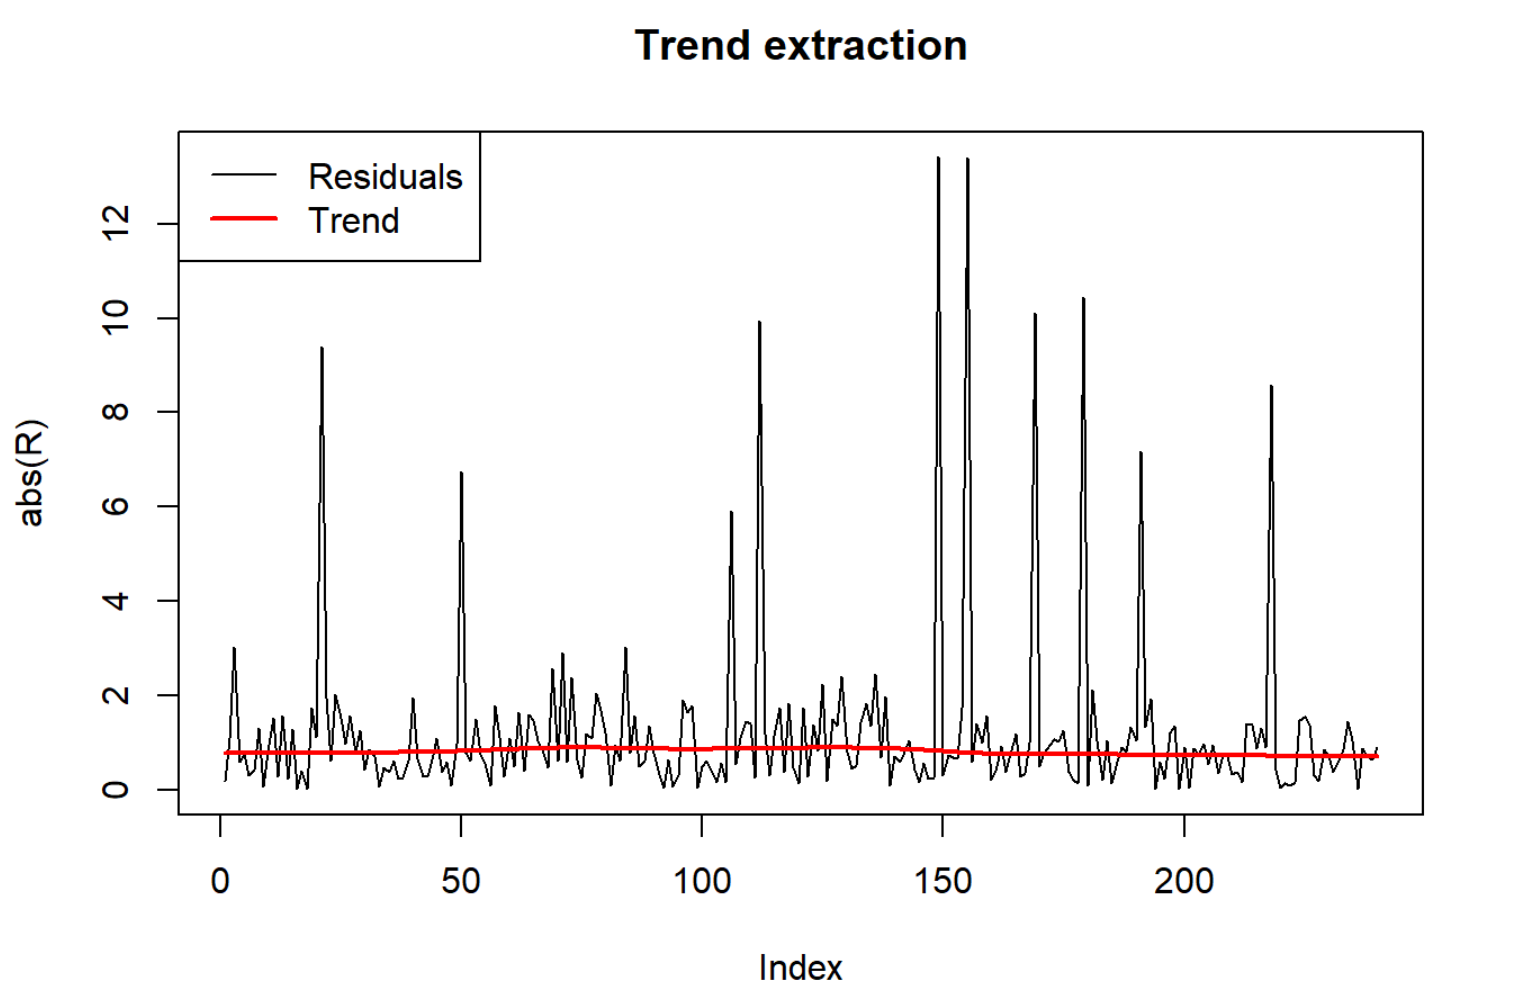
\includegraphics[width=1\linewidth]{Trend1}
\caption{ \footnotesize{График модуля остатков. Постоянная дисперсия шума.}} %% подпись к рисунку
\label{ris:experimoriginal} %% метка рисунка для ссылки на него
\end{minipage}
\hfill
\begin{minipage}[h]{0.47\linewidth}
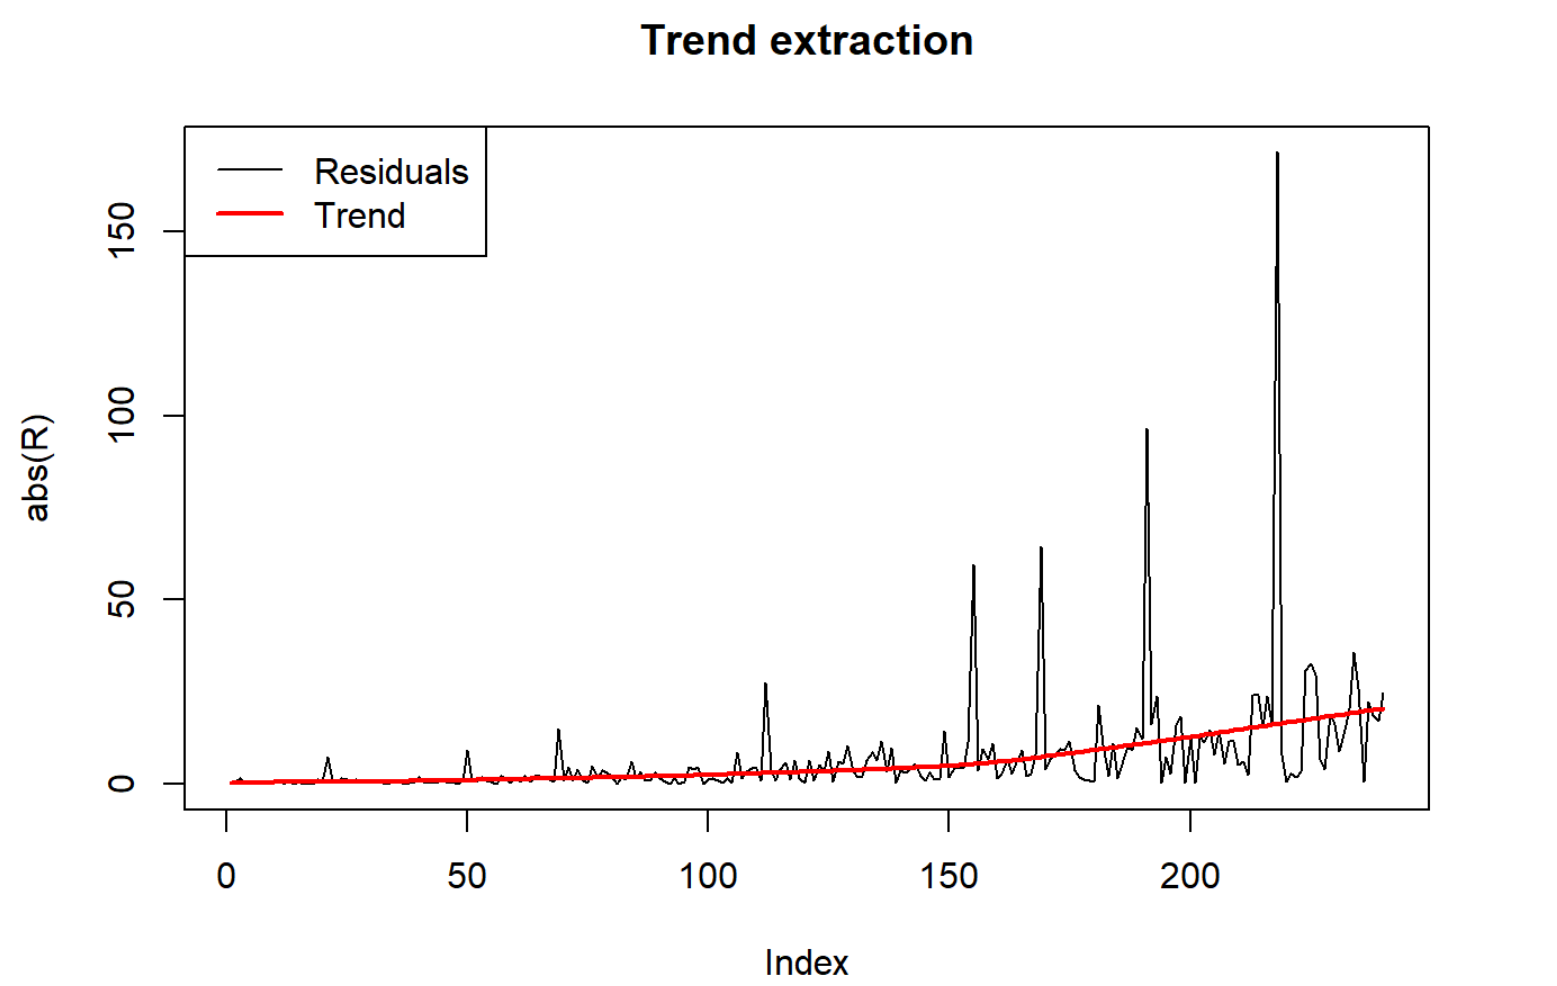
\includegraphics[width=1\linewidth]{Trend2}
\caption{\footnotesize{График модуля остатков. Гетероскедастичный шум.}}
\label{ris:experimcoded}
\end{minipage}
\end{center}
\end{figure}}
\footnotesize
\textbf{Решение}: Будем рассматривать матрицу $\bm{\Sigma} = \{\sigma_{ij}\}_{i,j=1}^{L,K}$ ганкелевой, что соответствует приписыванию весов элементам ряда. Обозначим параметр $\bm{\sigma} = (\sigma_1,\ldots,\sigma_N)^\mathrm{T}$. Будем задавать параметр $\bm{\sigma}$ как тренд (мат. ожидание) ряда, состоящего из модулей остатков.

\note{
	Авторы алгоритма предлагают выбрать $\sigma_{ij}$ не зависящими от $i,~j$. Однако такой выбор не подходит, к примеру, для рядов с гетероскедастичным шумом. 
	Нормировка остатков на константный параметр $\sigma_{ij} = \sigma~ \forall i,j$ в случае шума с непостоянной дисперсией приводит к неправильной идентификации точек с выбросами. Если
	шум растет к концу ряда, то веса у всех значений на конце ряда некорректно занижаются,
	и точки, не содержащие выбросов, могут получить вес, меньший, чем у выбросов
	в начале ряда. Поэтому приходим к выводу, что нормирующий параметр необходимо
	задавать динамически.
	
	Будем рассматривать матрицу $\bm{\Sigma} = \{\sigma_{ij}\}_{i,j=1}^{L,K}$ ганкелевой, что соответствует приписыванию весов элементам ряда. В модификации метода предполагается замена параметра $\sigma_{ij}$ на элементы траекторной матрицы тренда (оценки математического ожидания) ряда, состоящего из модулей остатков. Выделять тренд будем следующими способами: локальной регрессией loess, скользящей медианой или взвешенной локальной регрессией lowess.
}
\end{frame}

\begin{frame}
\frametitle{WL2-SSA. Выбор параметров. Параметр $\alpha$}
\footnotesize{
\textbf{Проблема 2}:
Непонятно, как задавать параметр $\alpha$, влияющий на то, какие точки считать выбросами, а какие --- нет. 

\textbf{Решение}: 
Выведем вероятностную формулу для параметра $\alpha$. 

Модель ряда: $x_i=s_i+\varepsilon_i,$ $i=1,\ldots,N$. Ганкелизуем матрицу остатков $\mathbf{R}= \mathbf{Y} - \mathbf{U}\mathbf{V}^{\mathrm{T}}$, получим ряд $\tX{R}=\{r_i\}_{i=1}^N$. В предположении точной отделимости сигнала от шума, ряд $\tX{R}=\{\varepsilon_i\}_{i=1}^N$.
Будем задавать вероятность $\gamma$: $\mathrm{P}(r^*\in (0,\alpha))=\gamma$, где $r^*=\frac{|\varepsilon|}{\sigma}$, $\bm{\sigma} =(\sigma_1,\ldots,\sigma_N)$ --- тренд из ряда $|\tX{R}|$.

\begin{definition}
	%Пусть $R=(r_1,\ldots,r_q)^\mathrm{T}$. 
	\footnotesize Если $r \sim N(0, \sigma^2)$, то $|r| \sim N_{H}(\sigma^2)$ --- \alert{полунормальное распределение} с параметром $\sigma^2$, ф.р.
	$F_H(x;\sigma^2) = \frac{2}{\sqrt{\pi}}\int\limits_{0}^{x/\sqrt{2}\sigma^2} e^{-z^2} dz = \text{erf} (\frac{x}{\sqrt{2}\sigma^2})$.
	%среднее $\mathbb{E}|r|=\sigma \sqrt{\frac{2}{\pi}},$ дисперсия $ \mathbb{D}|r|=\sigma^2 (1-\frac{2}{\pi})$.
\end{definition}
\begin{proposition}
	\footnotesize Пусть $\varepsilon\sim N(0,\sigma_{\varepsilon}^2)$, $\sigma=\E |\varepsilon|$. Тогда $r^{*}=\frac{|\varepsilon|}{\sigma}$ имеет полунормальное распределение $N_H(\frac{\pi}{2}),$ среднее $\E r^* = 1,$ дисперсия $\D r^* = \frac{\pi}{2}-1$.
\end{proposition}
Получаем выражение для $\alpha$:
\begin{equation*}
\alpha = \frac{\sqrt{2}\pi}{2} \text{erf}^{-1}(\gamma).
\end{equation*}
%К примеру, для $\gamma = 0.95$ получим $\alpha \approx 3.079$. Для $\gamma = 0.99$: $\alpha \approx 4.046$.
\alert{Замечание:}
	В предположении нормальности шума и точной отделимости сигнала от шума формула верна и для нестационарного шума.  %$r^* \sim N_H(\frac{\pi}{2}).$
}
\note{
	\small{
	У метода с итеративным обновлением весов есть параметр $\alpha$, который влияет на
	то, какие точки будем считать выбросами, а какие --- нет. Для того, чтобы понять, какое
	значение следует взять в качестве $\alpha$, выведем вероятностную формулу для этого
	параметра. Для вывода формулы введем определение полунормального распределения. 
	
	Напомним, что мы рассматриваем ряд, который является суммой сигнала и шума.
	Если предположить точную отделимость сигнала от шума, то ряд из остатков соответствует шуму.  Обозначим $r^* = \frac{|\varepsilon|}{\sigma}$, где $\sigma$ --- компонента тренда ряда из модулей остатков.  
	Мы хотим задавать вероятность $\gamma$ так, чтобы нормированные модули остатков попадали в промежуток $(0;\alpha)$ с вероятностью $\gamma$. Для того, чтобы получить выражение для $\alpha$, нам необходимо знать распределение $r^*$. Можно показать, что $r^*$ имеет полунормальное распределение с параметром $\frac{\pi}{2}$. Тогда можем вывести формулу для параметра $\alpha$, она представлена на слайде. Также можно заметить, что утверждение и выведенная формула верны не только для шума постоянной дисперсии, но и для гетероскедастичного шума.
}
}
\end{frame}


%\begin{frame}
%\frametitle{WL2-SSA. Метод с итеративным обновлением весов. Параметр $\alpha$}
%Модель ряда: $x_i=s_i+\varepsilon_i,$ $i=1,\ldots,N$.
%
%\small
%Ганкелизуем матрицу остатков $\mathbf{R}= \mathbf{Y} - \mathbf{U}\mathbf{V}^{\mathrm{T}}$, получим ряд $\tX{R}=\{r_i\}_{i=1}^N$. Если матрица $\mathbf{R}$ соответствует траекторной матрице шума $\{\varepsilon_i\}_{i=1}^N$, то ряд $\tX{R}=\{r_i\}_{i=1}^N=\{\varepsilon_i\}_{i=1}^N$.
%Обозначим $r^*=\frac{|\varepsilon|}{\sigma}$, где $\bm{\sigma} =(\sigma_1,\ldots,\sigma_N)$ --- тренд из ряда $|\tX{R}|$. Хотим задавать вероятность $\gamma$: $\mathrm{P}(r^*\in (0,\alpha))=\gamma$.
%
%%\begin{equation*}
%%\mathrm{P}(\eta\in (0,\alpha))=\mathrm{P}(0\le \frac{|\varepsilon|}{\sigma} \le \alpha) = \mathrm{P}(\frac{|\varepsilon|}{\sigma} \le \alpha) = \gamma.
%%\end{equation*}
%
%\begin{proposition}
%	\small Пусть $\varepsilon\sim N(0,\sigma_{\varepsilon}^2)$, $\sigma=\E |\varepsilon|$. Тогда $r^{*}=\frac{|\varepsilon|}{\sigma_{\varepsilon}}$ имеет полунормальное распределение $N_H(\frac{\pi}{2}),$ среднее $\E r^* = 1,$ дисперсия $\D r^* = \frac{\pi}{2}-1$.
%\end{proposition}
%Получаем выражение для $\alpha$:
%\begin{equation*}
%\alpha = \frac{\sqrt{2}\pi}{2} \text{erf}^{-1}(\gamma).
%\end{equation*}
%К примеру, для $\gamma = 0.95$ получим $\alpha \approx 3.079$. Для $\gamma = 0.99$: $\alpha \approx 4.046$.
%\begin{notice}
%	Как в случае шума постоянной дисперсии, так и в случае гетероскедастичного шума, в предположении нормальности шума и точной отделимости сигнала от шума, $r^*$ имеет полунормальное распределение $N_H(\frac{\pi}{2}).$
%\end{notice}
%\note{
%  Напомним, что мы рассматриваем ряд, который является суммой сигнала и шума.
%  Если предположить точную отделимость сигнала от шума, то матрица остатков соответствует траекторной матрице шума. Для случайного шума мы не можем наблюдать точную отделимость, однако будем предполагать разделимость в дальнейших рассуждениях. Тогда ряд из остатков соответствует шуму.  Обозначим $r^* = \frac{|\varepsilon|}{\sigma}$, где $\sigma$ --- компонента тренда ряда из модулей остатков. В предположении точной отделимости это
%  означает, что $\sigma_i = \E|\varepsilon_i|$. 
%  
%  Мы хотим задавать вероятность $\gamma$ так, чтобы $r^*$ попадало в промежуток $(0;\alpha)$ с вероятностью $\gamma$. Для того, чтобы получить выражение для $\alpha$, нам необходимо знать распределение $r^*$. Можно показать, что $r^*$ имеет полунормальное распределение с параметром $\frac{\pi}{2}$, среднее равно 1, а дисперсия равна $\frac{\pi}{2}-1$. Тогда можем вывести формулу для параметра $\alpha$, она представлена на слайде. Также можно заметить, что утверждение и выведенная формула верны не только для шума постоянной дисперсии, но и для гетероскедастичного шума.
%}
%\end{frame}

%\begin{frame}
%\frametitle{Метод с итеративным обновлением весов. Параметр $\alpha$}
%
%\begin{notice}
%\small Пусть шум гетероскедастичный, $\alert{x_i= s_i + t_i\varepsilon_i},$ где $t_i>0$, $\varepsilon_i\sim N(0,1)$, сигнал $s_i$ известен. Пусть $\tX{R}=(r_1,\ldots,r_N)^\mathrm{T}$ --- остатки, $\tX{R}_+=(|r_1|, \ldots, |r_N|)^\mathrm{T}$ --- вектор из модулей остатков, $\bm{\sigma}=(\sigma_1,\ldots,\sigma_N)^\mathrm{T} = \mathbb{E}(\tX{R}_+)$. Тогда каждая компонента вектора $\tX{r}^*=(\frac{|r_1|}{\sigma_1}, \ldots, \frac{|r_N|}{\sigma_N})^\mathrm{T}$ имеет полунормальное распределение: $r_i^* = \frac{|r_i|}{\sigma_i} \sim N_H(\frac{\pi}{2})$. В таком случае $\E r_i^* = 1,$ $\D r_i^* = \frac{\pi}{2}-1$.
%\end{notice}
%
%%\begin{notice}
%%	\small Пусть шум гетероскедастичный, $\alert{x_i= s_i + t_i\varepsilon_i},$ где $t_i>0$, $\varepsilon_i\sim N(0,1)$, сигнал $s_i$ известен. Пусть $\tX{R}=(r_1,\ldots,r_N)^\mathrm{T}$ --- остатки, $\tX{R}_+=(|r_1|, \ldots, |r_N|)^\mathrm{T}$ --- вектор из модулей остатков, $\bm{\sigma}=(\sigma_1,\ldots,\sigma_N)^\mathrm{T} = \mathbb{E}(\tX{R}_+)$. Тогда каждая компонента вектора $\tX{r}^*=(\frac{|r_1|}{\sigma_1}, \ldots, \frac{|r_N|}{\sigma_N})^\mathrm{T}$ имеет полунормальное распределение: $r_i^* = \frac{|r_i|}{\sigma_i} \sim N_H(\frac{\pi}{2})$. В таком случае $\E r_i^* = 1,$ $\D r_i^* = \frac{\pi}{2}-1$.
%%\end{notice}
%\small
%%Тогда уравнение $\mathrm{P}(\frac{|\varepsilon|}{\sigma} \le \alpha) = \gamma$ эквивалентно $F_H(\alpha) = \gamma$, где $F_H$ --- функция распределения $N_H(\frac{\pi}{2})$.
%%Получаем выражение для $\alpha$:
%%\begin{equation*}
%%\alpha = \frac{\sqrt{2}\pi}{2} \text{erf}^{-1}(\gamma).
%%\end{equation*}
%%К примеру, для $\gamma = 0.95$ получим $\alpha \approx 3.079$. Для $\gamma = 0.99$: $\alpha \approx 4.046$. \\
%%~~\\
%\end{frame}
\begin{frame}
\frametitle{WL2-SSA. Метод с итеративным обновлением весов. Реализация}
\alert{Алгоритм IRLS} (параметры $\alpha$ и $\sigma$) [Chen K., Sacchi M., 2015]:\\
\footnotesize {
	\begin{enumerate}
		\item Инициализация $\mathbf{U}\in \mathbb{R}^{L\times r}$ и $\mathbf{V}\in \mathbb{R}^{K\times r}$ (например, с помощью сингулярного разложения матрицы $\mathbf{Y}$),
		\item Выбор параметра $\alpha$ (величина, начиная с которой точку ряда считать выбросом),
		\item  Вычисление матрицы остатков $\mathbf{R}=\{r_{ij}\}_{i,j=1}^{L,K} = \mathbf{Y}-\mathbf{U}\mathbf{V}^{\mathrm{T}}$,
		\item  Обновление параметра $\sigma_{ij}$ (нормировка для остатков),
		\item Вычисление матрицы весов $\mathbf{W} = \{w_{ij}\}_{i,j=1}^{L,K} = \{w(\frac{r_{ij}}{\sigma_{ij}})\}_{i,j=1}^{L,K} $, используя %$w(x)=\frac{\partial \rho(x)}{\partial |x|} \frac{1}{|x|}$:
		\begin{equation*}
		w(x) = 
		\begin{cases}
		(1-(\frac{|x|}{\alpha})^2)^2, &|x|\le\alpha\\
		0, &|x|>\alpha
		\end{cases},% ~~~~\text{где}~ x=\frac{1}{\sigma}r,
		\end{equation*}
		\item Решение задачи взвешенной аппроксимации (обновление матриц $\mathbf{U}$ и $\mathbf{V}$)
		\begin{equation*}
		\norm{\mathbf{W}^{1/2}\odot(\mathbf{Y}-\mathbf{U}\mathbf{V}^{\mathrm{T}})}^2_F \longrightarrow \min_{\mathbf{U},\mathbf{V}}.
		\end{equation*}	
		
		\item Повторяем шаги 3--6, пока не выполнен критерий сходимости
		\begin{equation*}
		\norm{\mathbf{W}^{1/2}\odot(\mathbf{Y}-\mathbf{U}\mathbf{V}^{\mathrm{T}})}^2_F \le \varepsilon
		\end{equation*} 
		или не достигнуто максимальное число итераций $N_{IRLS}$.
	\end{enumerate}
}
\note{
Посмотрим еще раз на алгоритм оригинального метода с обновлением весов. Модификация отличается от оригинального метода пятым пунктом.
}
\end{frame}

\begin{frame}
\frametitle{WL2-SSA. Метод с итеративным обновлением весов. Модификация}
Модификация 5-ого пункта алгоритма IRLS:\\
\begin{enumerate}
\item [5.a]  Ганкелизация матрицы $\mathbf{R}$ и получение ряда длины $N$ из остатков: $\tX{R} = \mathcal{T}^{-1} \Pi_{\mathcal{H}} (\mathbf{R}) = (r_1,\ldots,r_N)^\mathrm{T}$,
\item [5.b] Пусть $\tX{R}_+=(|r_1|, \ldots, |r_N|)^\mathrm{T}$ --- вектор из модулей остатков. Вычисление $\bm{\sigma} = (\sigma_1,\ldots,\sigma_{N})^\mathrm{T}$ как оценки мат. ожидания $\mathbb{E}(\tX{R}_+)$ некоторым выбранным методом,
\item [5.c]  Вычисление ряда $|\bm{\sigma}^{-1}\tX{R}| = (\frac{|r_1|}{\sigma_1},\ldots,\frac{|r_N|}{\sigma_N})^\mathrm{T}$ и получение матрицы $\mathbf{R}^{*} = \{r_{ij}^*\}_{i,j=1}^{L,K} = \mathcal{T} (|\bm{\sigma}^{-1}\tX{R}|)$,
\item [5.d] Вычисление матрицы весов $\mathbf{W}= \{w_{ij}\}_{i,j=1}^{L,K} = \{w(r_{ij}^*)\}_{i,j=1}^{L,K}$, используя %$w(x)=\frac{\partial \rho(x)}{\partial |x|} \frac{1}{|x|}$:
\begin{equation*}
w(x) = 
\begin{cases}
(1-(\frac{|x|}{\alpha})^2)^2, &|x|\le\alpha\\
0, &|x|>\alpha
\end{cases}. %~~~ \text{где}~ x=r^*.
\end{equation*} 
\end{enumerate}
\note{
	 В модификации алгоритма после вычисления матрицы остатков мы должны ее ганкелизовать, получив ряд из остатков. Затем вычислить некоторым методом тренд (оценку мат. ожидания) из ряда, состоящего из модулей остатков, и нормировать модули на вычисленный тренд. Построив траекторную матрицу получившегося ряда, мы	получаем новую матрицу остатков, и далее применяем функцию весов уже к этой матрице.
	
	Тренд будем выделять следующими способами: с помощью локальной регрессии loess, скользящей медианой или с помощью взвешенной локальной регрессии lowess.
}
\end{frame}

\begin{frame}
\frametitle{Сравнение теоретических трудоемкостей}
Ряд $\tX{X}=(x_1, \ldots, x_{N})$ длины $N$, матрица $\mathbf{Y}\in \mathbb{R}^{L\times K}$ --- траекторная матрица ряда $\tX{X}$. Ранг траекторной матрицы сигнала равен $r$.
\begin{itemize}
\item Трудоемкость последовательного метода: 
\begin{equation*}
\mathrm{T}_{\mathrm{l1pca}} = O(LK\log (2LK+Lr)N_{iter}),
\end{equation*}
где $N_{iter}$ — общее кол-во итераций для сходимости метода (по выбранному критерию сходимости).

\item Трудоемкость метода с обновлением весов: 
\begin{equation*}
\mathrm{T}_{\mathrm{IRLS}} = O(LKr^2N_\alpha N_{IRLS}),
\end{equation*}
где $N_\alpha$ и $N_{IRLS}$ — общее кол-во итераций для решения задач (\ref{taskA}), (\ref{taskB}) и сходимости метода (по выбранному критерию сходимости).
\end{itemize}

%Вычислительные эксперименты показали, что максимальное число итераций для последовательного метода $N_{iter}$ достаточно взять равным 5, $N_\alpha$ и $N_{IRLS}$ --- 5 и 10 соответственно (отличия в ошибках восстановления сигнала при увеличении итераций незначительны, ~~ ошибка уменьшается не более чем на $0.2 \%$).
Число итераций в статьях предполагается фиксированным. Однако предположение о достаточности фиксированного числа итераций не верно. В предположении, что число итераций не растет с увеличением длины ряда, так как зависит от разделимости, метод с итеративным обновлением весов оказывается менее трудоемким.
\note{
	Сравним теоретические трудоемкости рассмотренных методов. Трудоемкости последовательного метода и метода с обновлением весов представлены на слайде. 
	В трудоемкость входит число итераций, которое в статьях предполагается фиксированным.
	В работе показано, что предположение о достаточности фиксированного числа итераций
	не верно. Теоретически вывести достаточное число итераций не удалось. Однако,
	в предположении, что число итераций не растет с увеличением длины ряда, так как
	зависит от разделимости, которая только улучшается, удалось теоретически сравнить
	трудоемкости. Метод с итеративным обновлением весов оказался менее трудоемким. 
}
\end{frame}

%\begin{frame}
%\frametitle{Сравнение теоретических трудоемкостей}
%Ряд $\tX{X}=(x_1, \ldots, x_{N})$ длины $N$, матрица $\mathbf{Y}\in \mathbb{R}^{L\times K}$ --- траекторная матрица ряда $\tX{X}$. Ранг траекторной матрицы сигнала равен $r$.
%Трудоемкости методов:
%\begin{itemize}
%\item$\mathrm{T}_{\mathrm{l1pca}} = O(LK\log (2LK+Lr)N_{iter})$,
%\item $\mathrm{T}_{\mathrm{IRLS}} = O(LKr^2N_\alpha N_{IRLS})$.
%\end{itemize}
%~~\\
%Рассмотрим 2 случая:
%\begin{itemize}
%\item Траекторная матрица вытянута, $L$ мало, фиксировано, $K = N-L+1 \sim N$. Асимптотически трудоемкость метода с весами IRLS оказывается меньше. 
%
%\item Траекторная матрица ряда близка к квадратной, $L\sim\frac{N}{2}, K\sim\frac{N}{2}$.
%И в этом случае асимптотически трудоемкость метода с весами IRLS оказывается меньше. 
%\end{itemize}
%~~\\
%\alert{Вывод}: асимптотически теоретическая трудоемкость метода IRLS оказывается меньше.
%\end{frame}


\begin{frame}
\frametitle{Вычислительный эксперимент. Структура исследования}
Пусть длина ряда $N=240$. Рассмотрим следующие примеры: 
\begin{enumerate}
\item $x_n= e^{n/N}+\sin{(2\pi n/120+\pi/6)}+\varepsilon_n, ~~~ \varepsilon_n \sim N(0,1)$,  $r=3$,
\item $x_n=e^{4n/N} \sin(2\pi n/30) + Ae^{4n/N}\varepsilon_n, ~~~~~~ \varepsilon_n \sim N(0,1)$,  $r=2$,
\item $x_n= ne^{4n/N}\sin{(2\pi n/30)}+\varepsilon_n, ~~~~~~~~~~~~~ \varepsilon_n \sim N(0,1)$,  $r=4$.
\end{enumerate}	
Выбросы: в случайно выбранных точках ряда $x_i$ значение заменяется на $x_i + \delta x_i$, где $\delta$ --- заданная константа.
\def\figurename{Пр. 1}
\begin{figure}[h]
\begin{center}
\begin{minipage}[h]{0.32\linewidth}
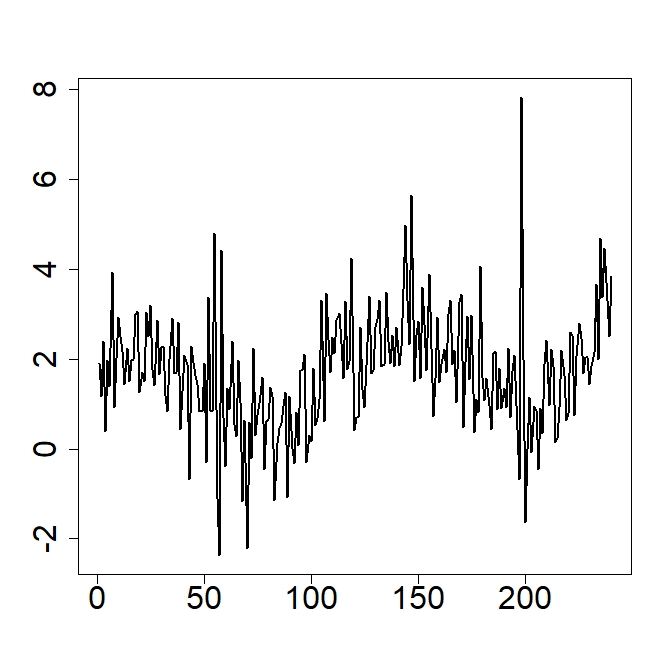
\includegraphics[width=1\linewidth]{SeriesPlot1}
\caption{1\% выбросов, выброс размера $5x_i$.} %% подпись к рисунку
\end{minipage}
\hfill
\def\figurename{Пр. 2}
\begin{minipage}[h]{0.32\linewidth}
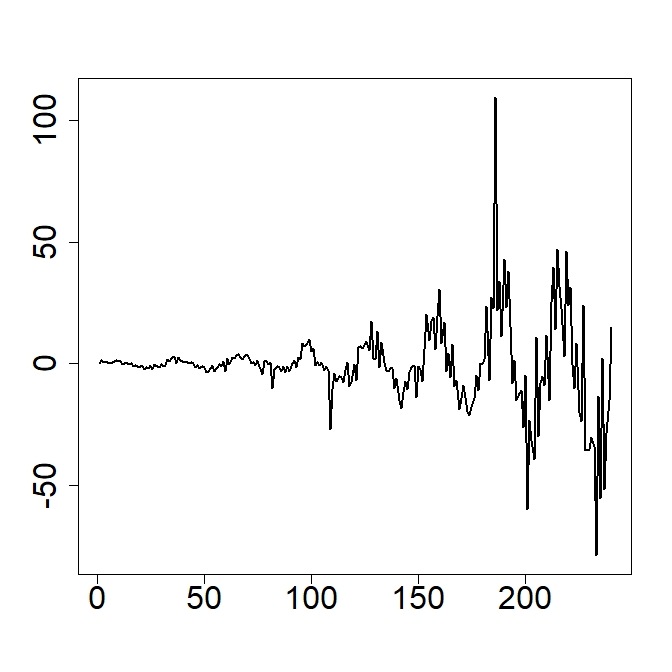
\includegraphics[width=1\linewidth]{SeriesPlot2}
\caption{1\% выбросов, выброс размера $5x_i$.}
\end{minipage}
\hfill
\def\figurename{Пр. 3}
\begin{minipage}[h]{0.32\linewidth}
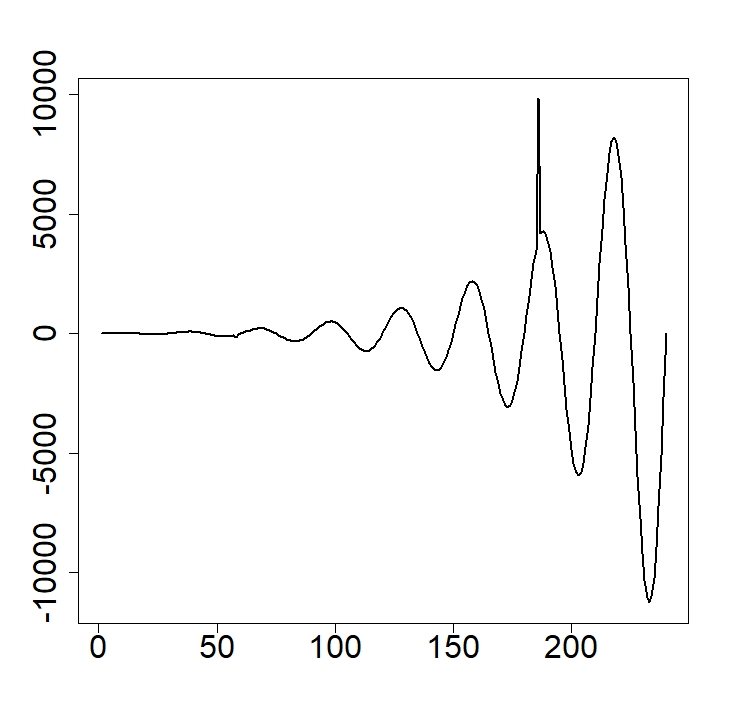
\includegraphics[width=1\linewidth]{SeriesPlot3}
\caption{1\% выбросов, выброс размера $1.5x_i$.}
\end{minipage}
\end{center}
\end{figure}
\def\figurename{Рис.}
\note{
	Рассмотрим 3 модельных примера. Формулы для рядов и графики с выбросами представлены на слайде. Выбросы добавляются следующим образом: случайных точках ряда к значению ряда $x_i$ добавляется  $\delta x_i$, где $\delta$ --- заранее заданная константа. 
}
\end{frame}


\begin{frame}
\frametitle{Вычислительный эксперимент. Структура исследования}
Временной ряд $\tX{X}=(x_1, \ldots, x_{N})$, $x_i = s_i + \varepsilon_i$, $i=1,\ldots,N$. Обозначим $\tX{S} = (s_1,\ldots,s_N)^\mathrm{T}$ --- сигнал. \\
~~\\
%Рассмотрим временной ряд 
%\begin{equation*}
%x_n= e^{n/N}+\sin{(2\pi n/120+\pi/6)}+\varepsilon_n, ~ \varepsilon_n \sim N(0,1),
%\end{equation*}	

\alert{Выбросы:} в случайно выбранных точках ряда $x_i$ значение заменяется на $x_i + \delta x_i$, где $\delta$ --- заданная константа. Будем сравнивать результаты при отсутствии (0\%) выбросов, при 1\% и 5\% выделяющихся наблюдений. \\
~~\\

На каждой реализации ряда случайными являются шум и местоположения выбросов. \\
~\\

Cравнения проводятся по величине ошибки, согласованной с $\mathbb{L}_2$ (MSE) и ошибки, согласованной с $\mathbb{L}_1$ (MAD):
\begin{equation*}
\text{\alert{MSE}}(\widetilde{\tX{S}},\tX{S}) = \mathbb{E} \left(\frac{1}{N} \sum \limits_{i=1}^{N}(s_i - \tilde s_i )^2 \right), ~~~ \text{\alert{MAD}}(\widetilde{\tX{S}},\tX{S}) = \mathbb{E} \left(\frac{1}{N} \sum \limits_{i=1}^{N}|s_i - \tilde s_i | \right),
\end{equation*}
где $\tX{S}$ --- сигнал, $\widetilde{\tX{S}}$ --- его оценка.
Будем вычислять \alert{RMSE} = $\sqrt{\textrm{MSE}}$. %Число повторов для оценок ошибок $M=100$.
\note{
	Будем сравнивать результаты при отсутствии выбросов, при 1\% и 5\% выбросов, которые будут находиться в случайных точках ряда.
	
	Сравнение будем проводить по величине ошибки MSE, согласованной с $\mathbb{L}_2$, и MAD, согласованной с $\mathbb{L}_1$. Из оценки ошибки MSE будем извлекать корень, получая RMSE.
}
\end{frame}


%\begin{frame}
%\frametitle{Вычислительный эксперимент. Структура исследования}
%В методе с итеративным обновлением весов необходимо задать параметры $\alpha$ и $\bm{\sigma}$. Для $\gamma = 0.99$ значение $\alpha$ получается  $4.046$. \\
%~~\\
%В качестве $\bm{\sigma}$ будем брать тренд из ряда остатков, выделение тренда будем проводить следующими способами:
%\begin{itemize}
%\item с помощью локальной регрессии loess с параметром сглаживания 0.35,
%\item скользящей медианой с длиной окна 80,
%\item с помощью взвешенной локальной регрессии lowess с параметром сглаживания 0.35. Это вариант локальной регрессии, где за несколько итераций с помощью добавления весов уменьшается влияние выбросов. 
%\end{itemize}
%\note{
%	Выберем параметры для метода с обновлением весов. Как было показано ранее, для $\gamma = 0.99$ значение параметра $\alpha = 4.046$. Стоит заметить, что такая вероятностная интерпретация параметра $\alpha$ верна только для модификации метода. 
%	
%	Выделение тренда будем проводить следующими способами:
%	с помощью локальной регрессии loess с параметром сглаживания 0.35, скользящей медианой с длиной окна 80 и с помощью взвешенной локальной регрессии lowess с параметром сглаживания 0.35. Это вариант локальной регрессии, где за несколько итераций с помощью добавления весов уменьшается влияние выбросов.
%}
%\end{frame}

%\begin{frame}
%\frametitle{Вычислительный эксперимент. Результаты}
%\begin{table}
%\caption{Оценки RMSE для трех примеров для $M=30$ реализаций ряда.}
%\label{tab_all}
%\centering
%\begin{tabular}{|c||c|c||c|c||c|c|}
%\hline
%&\multicolumn{2}{|c||}{Пример 1}& \multicolumn{2}{|c||}{Пример 2}&\multicolumn{2}{|c|}{Пример 3} \\
%\hline
%Method 	& 0\% & 5\% & 0\% & 5\% & 0\% & 5\% \\ 
%\hline
%Basic SSA & \textbf{\textcolor{red}{0.399}} & 0. 741  & \textbf{\textcolor{red}{1.76}}  & 4.71 & \textbf{\alert{0.201}} & 461.02 \\
%l1pca & 0.469 & \textbf{\alert{0.462}}  & \textbf{\alert{1.82}} & \textbf{\alert{1.94}} & 0.222 & 19.721\\
%IRLS (orig.) & 0.455 & \textbf{\textcolor{red}{0.444}}  & 2.67  & 2.69 & \textbf{\textcolor{red}{0.194}} & 301.2 \\
%IRLS (loess) & 0.490 & 0.497  & \textbf{\alert{1.79}} &  \textbf{\textcolor{red}{1.85}} &\textbf{\alert{0.197}} & 39.113 \\
%IRLS (median) & 0.511 & 0.530 & 2.31  & 2.42 & \textbf{\alert{0.209}} & 105.6 \\
%IRLS (lowess) & 0.495 & 0.499  &\textbf{\alert{2.09}} &  2.01 & \textbf{\alert{0.205}} & \textbf{\textcolor{red}{0.201}} \\
%\hline
%\end{tabular}
%\end{table}
%\small
%Проверка значимости сравнения по критерию для зависимых выборок:
%$\mathrm{H}_0: \mathbb{E}(\xi_1-\xi_2)=0$.
%Выборки $X=(x_1,\ldots,x_M)$ и $Y=(y_1,\ldots,y_M)$, $\bar{X}$ и $\bar{Y}$ --- их выб. средние, $s_x^2$ и $s_y^2$ --- выб. дисперсии, $\hat\rho$ --- коэффициент корреляции. 
%Статистика критерия 
%\begin{equation*}
%t = \frac{\sqrt{M}(\bar{X}-\bar{Y})}{\sqrt{s_x^2+s_y^2-2s_xs_y\hat\rho}} \xrightarrow []{d} N(0,1).
%\end{equation*}
%Уровень значимости $\alpha = 0.05$. В каждом столбце выделен наилучший метод \textcolor{red}{(красным)} и незначимо отличающиеся от него \alert{(синим)}.
%
%\note{
%	В таблице представлены оценки RMSE для трех примеров при 0\% и 5\% выбросов. Красным выделены методы, показавшие наименьшую ошибку, а синим --- методы, незначимо отличающиеся от лучших.
%	Сравнение проводилось по критерию для зависимых выборок при уровне значимости 0.05.
%}
%\end{frame}

\begin{frame}
\frametitle{Вычислительный эксперимент. Результаты}
%\begin{table}
%	\caption{Оценки RMSE для трех примеров для $M=10$ реализаций ряда.}
%	\label{tab_all}
%	\centering
%	\begin{tabular}{|c||c|c||c|c||c|c|}
%		\hline
%		&\multicolumn{2}{|c||}{Пример 1}& \multicolumn{2}{|c||}{Пример 2}&\multicolumn{2}{|c|}{Пример 3} \\
%		\hline
%		Method 	& 0\% & 5\% & 0\% & 5\% & 0\% & 5\% \\ 
%		\hline
%		Basic SSA & \textbf{\textcolor{red}{0.402}} & 0. 712  & \textbf{\textcolor{red}{1.72}}  & 4.85 & \textbf{\alert{0.203}} & 476.52 \\
%		l1pca & 0.477 & \textbf{\alert{0.459}}  & \textbf{\alert{1.80}} & \textbf{\alert{1.93}} & 0.228 & 21.270\\
%		IRLS (orig.) & 0.459 & \textbf{\textcolor{red}{0.440}}  & 2.63  & 2.70 & \textbf{\textcolor{red}{0.196}} & 398.2 \\
%		IRLS (loess) & 0.491 & 0.494  & \textbf{\alert{1.78}} &  \textbf{\textcolor{red}{1.87}} &\textbf{\alert{0.198}} & 54.212 \\
%		IRLS (median) & 0.520 & 0.528 & 2.24  & 2.41 & \textbf{\alert{0.213}} & 112.6 \\
%		IRLS (lowess) & 0.502 & 0.498  &\textbf{\alert{2.11}} &  2.03& \textbf{\alert{0.211}} & \textbf{\textcolor{red}{0.202}} \\
%		\hline
%	\end{tabular}
%\end{table}
\small{
\begin{table}
\caption{Оценки RMSE для трех примеров для $M=30$ реализаций ряда.}
\label{tab_all}
\centering
\begin{tabular}{|c||c|c||c|c||c|c|}
\hline
&\multicolumn{2}{|c||}{Пример 1}& \multicolumn{2}{|c||}{Пример 2}&\multicolumn{2}{|c|}{Пример 3} \\
\hline
Method 	& 0\% & 5\% & 0\% & 5\% & 0\% & 5\% \\ 
\hline
Basic SSA & \textbf{\textcolor{red}{0.184}} & 0.653  & \textbf{\textcolor{red}{2.16}}  & 5.96 & \textbf{\textcolor{red}{0.215}} & 459.6 \\
l1pca & 0.217 & 0.250  & \textbf{\alert{2.45}} & 2.87 & 0.256 & 21.11\\
IRLS (orig.) & \textbf{\textcolor{red}{0.184}} & \textbf{\alert{0.206}}  & 3.52  & 3.61 & \textbf{\alert{0.216}} & 398.2 \\
IRLS (loess) & 0.196 & \textbf{\textcolor{red}{0.204}}  & \textbf{\alert{2.31}} &  \textbf{\textcolor{red}{2.39}} &\textbf{\alert{0.227}} & 303.2 \\
IRLS (median) & 0.210 & 0.223 & 2.84  & 2.86 & 0.256 & 38.21 \\
IRLS (lowess) & 0.206 & \textbf{\alert{0.211}}  & 2.59 &  2.63 & 0.243 & \textbf{\textcolor{red}{0.301}} \\
\hline
\end{tabular}
\end{table}
}
\small{
В каждом столбце выделен наилучший метод \textcolor{red}{(красным)} и незначимо отличающиеся от него \alert{(синим)} при уровне значимости $\alpha = 0.05$.
Выводы:
\begin{itemize}
\item Для первого примера наиболее устойчивыми являются оригинальный метод IRLS и его модификации с loess и lowess.
\item Для ряда с гетероскедастичным шумом наиболее устойчивый метод~---~модификация IRLS с использованием локальной регрессии.
\item В случае быстрорастущей амплитуды ряда модификация с использованием взвешенной локальной
регрессии оказывается наиболее устойчивой.
\end{itemize}
}

\note{
	Результаты вычислительного эксперимента для модельных примеров представлены в таблице. В каждом столбце красным выделен метод, показавший наименьшую ошибку, а синим --- незначимо отдичающиеся от него при уровне значимости 0.05. Проверка значимости проводилась по критерию для зависимых выборок, число реализаций ряда было взято равным 30.
	
	Можно сделать следующие выводы. Для примера без растущей амплитуды ряда и с шумом постоянной дисперсии наиболее устойчивыми являются оригинальный метод с обновлением весов и его модификации с использованием локальной регрессии loess и взвешенной локальной регрессии lowess. Для ряда с гетероскедастичным шумом преимущество оригинального метода с обновлением весов IRLS пропадает, наиболее устойчивым методом оказывается модификация IRLS с использованием локальной регрессии. В случае быстрорастущей амплитуды ряда модификация с использованием взвешенной локальной регрессии оказывается наиболее устойчивой.
}
\end{frame}

\begin{frame}
\frametitle{Реальный пример}
\small{
Рассмотрим ряд — импорт товаров в США из Кувейта с ноября 1993~г. по ноябрь 2012~г.. Имеются
данные за каждый месяц. Длина ряда $N = 229$. Возьмем длину окна $L=60$, будем восстанавливать сигнал по $5$ компонентам. \\
~~\\

Выбросы находятся в точках $x_{83}$ и $x_{222}$. В качестве истинного сигнала будем брать результат восстановления сигнала стандартным SSA для ряда с поставленными на места выбросов и впоследствии заполненными пропусками.
}
\begin{figure}[!h]
	\center{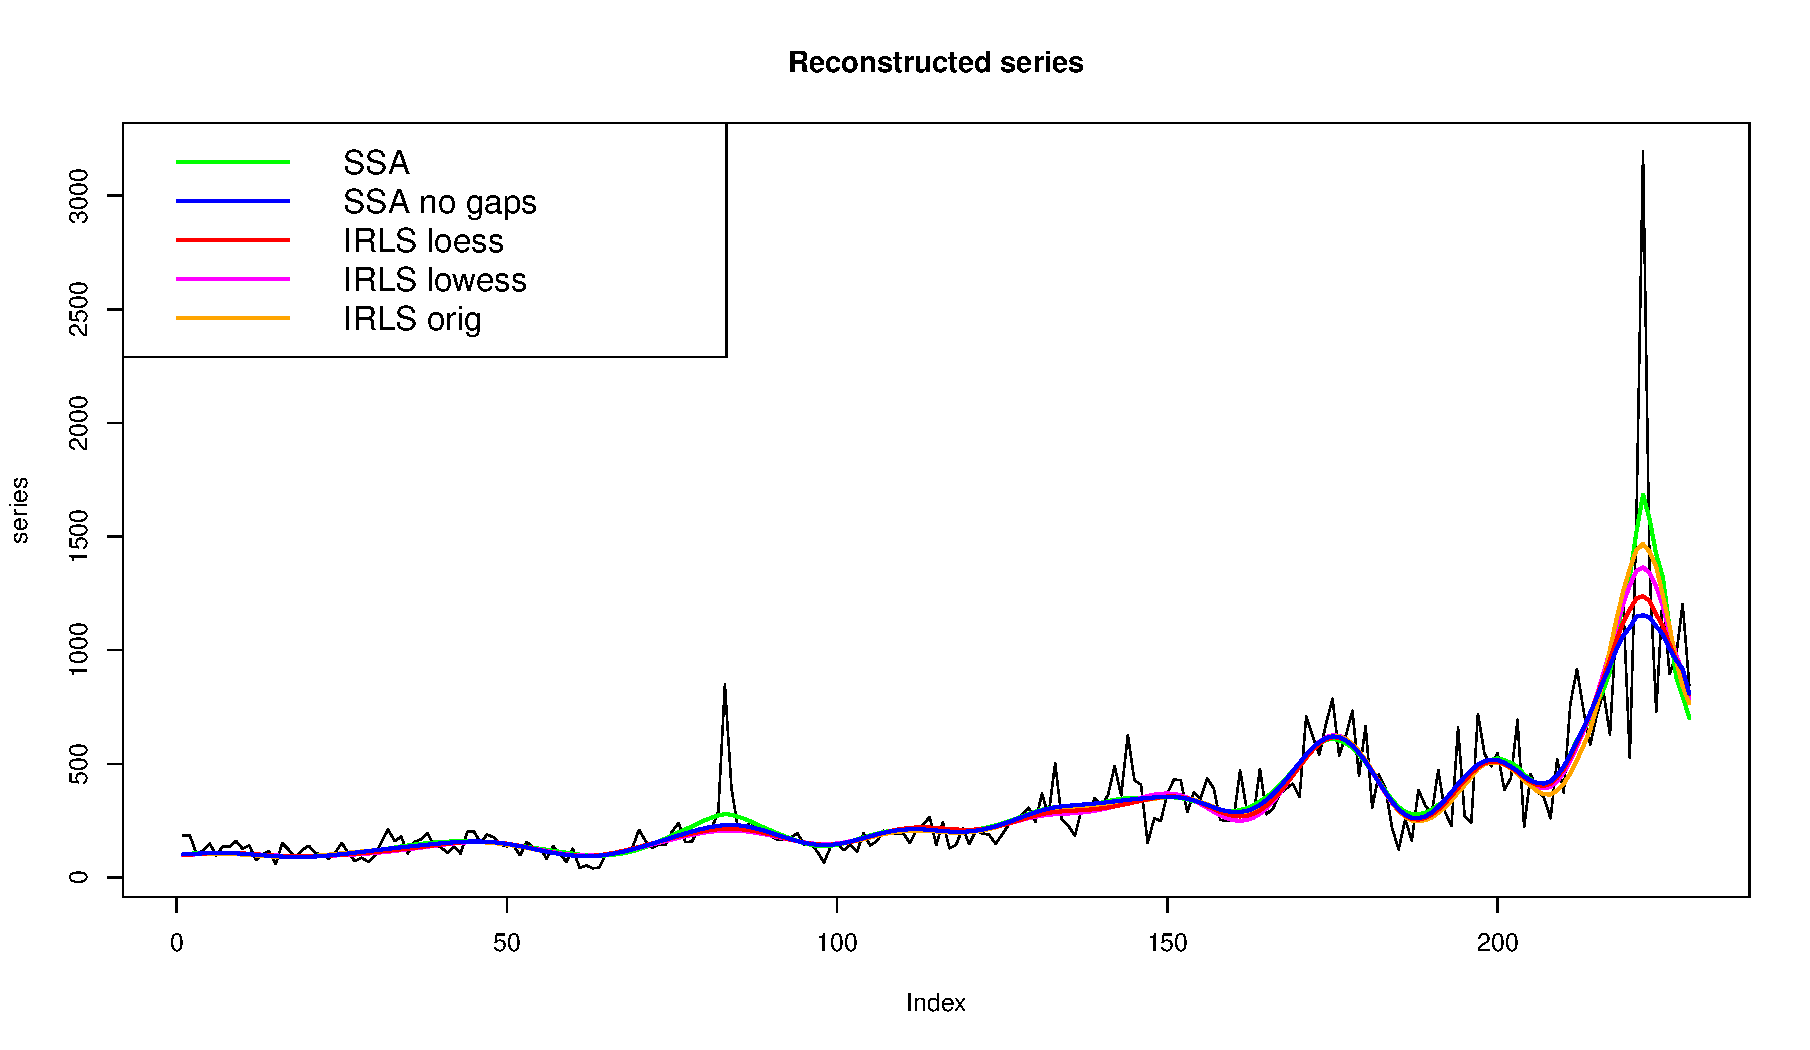
\includegraphics[width=0.75\linewidth]{Real_result1}}
	%\caption{Результат восстановления сигнала различными методами.}
	\label{Real}
\end{figure}
\note{
	\small{
	Продемонстрируем работу методов на реальном примере. Рассмотрим ряд --- импорт товаров в США из Кувейта с ноября 1993 года по ноябрь 2012 года с данными за каждый месяц. Возьмем длину окна $L = 60$. Проанализировав графики элементарных восстановленных рядов и матрицу взвешенных корреляций, был сделан вывод, что восстанавливать сигнал необходимо по первым 5 компонентам.
	Так как настоящий сигнал нам неизвестен, то попробуем на месте выбросов поставить пропуски, заполнить пропущенные значения, а затем выделить сигнал с помощью классического SSA. Полученный сигнал будем считать истинным. Сравним стандартный SSA и оригинальный метод с обновлением весов с предложенными модификациями (с выделением тренда с помощью локальной регрессии loess и взвешенной локальной регрессии lowess). 
	~~\\
	Результат восстановления сигнала различными методами представлен на рисунке. Можно заметить, что стандартный метод с обновлением весов (оранжевая линия) плохо справляется с выбросом на конце ряда, где дисперсия шума увеличивается. Наиболее близким к "истинному"$~$сигналу оказывается модификация с использованием loess (красная линия).
}
}
\end{frame}

%\begin{frame}
%\frametitle{Вычислительный эксперимент. Результаты. Пример 3}
%Рассмотрим 3 пример. Пусть присутствует всего один выброс в фиксированной точке ряда. Красным отмечены точки ряда с большой амплитудой, в которых присутствие выброса сильно искажает ряд.
%\begin{table}
%\caption{RMSE в зависимости от положения выброса для устойчивых методов (пример 3).}
%\centering
%\begin{tabular}{|c||c|c|c|c|c|c|c|}
%\hline
%Method 	& $x_{50}$ & $x_{100}$ & \textcolor{red}{$x_{173}$} & \textcolor{red}{$x_{203}$} & $x_{210}$ & \textcolor{red}{$x_{220}$} & \textcolor{red}{$x_{235}$}\\ 
%\hline
%%	Basic SSA & 0.31 & 65.3 & 4.387275e+03 & 3.15e+04 & 5.84 & 8.62e+04 & 3.95e+05 \\
%l1pca & 0.30 & 0.36 & 0.32 & 0.31 & 0.34 & 2.70 & 4.33 \\
%IRLS (orig.) &  0.25 & 0.27 & 0.83 & 0.61 & 0.60 & 4.21 & 16.1 \\
%IRLS (loess) &  0.21 & 0.23 & 0.71 & 0.52 & 0.40 & 1.13 & 7.21 \\
%IRLS (median) &  0.23 & 026. & 0.79 & 0.58 & 0.55 & 2.07 & 9.40 \\
%IRLS (lowess) & 0.20 & 0.21 & 0.25 & 0.31 & 0.24 & 0.27 & 0.35 \\
%
%\hline
%\end{tabular}
%\end{table}
%
%Вывод:
%\begin{itemize}
%\item Если выброс попадает в точку ряда с очень большой амплитудой, ошибки методов l1pca и IRLS (loess) увеличиваются. Метод IRLS с выделением тренда с помощью lowess оказывается в этом случае устойчивее.
%
%\end{itemize}
%\end{frame}

%\begin{frame}
%\frametitle{Результаты применения устойчивых методов к ряду}
%\small
%\begin{figure}[h]
%	\begin{minipage}[h]{0.49\linewidth}
%		\center{\includegraphics[width=1.09\linewidth]{RecSeries_end} \\ }
%	\end{minipage}
%	\hfill
%	\begin{minipage}[h]{0.49\linewidth}
%		\center{\includegraphics[width=1.0\linewidth]{RecError_endAbs} \\}
%	\end{minipage}
%	\caption{Результаты восстановления сигнала и модуль ошибок восстановления в присутствии выброса в одной точке ряда $x_{150}$.}
%\end{figure}
%
%\begin{table}
%	%\caption{RMSE в зависимости от положения выброса для устойчивых методов (пример 3).}
%	\centering
%	\begin{tabular}{|c|c|c|c|c|}
%		\hline
%		 Method & SSA  & l1pca & IRLS (loess) & IRLS (orig.) \\ 
%		\hline
%	      RMSE & 0.310 & 0.275 & 0.270 & 0.230  \\		
%		\hline
%	\end{tabular}
%\end{table}
%В случае выброса лишь в одной точке ряда один из вариантов IRLS выдал ошибку, меньшую, чем у SSA. 
%\end{frame}

%\begin{frame}
%\frametitle{Результаты применения устойчивых методов к ряду}
%\small
%\begin{figure}[h]
%\begin{minipage}[h]{0.49\linewidth}
%\center{\includegraphics[width=1.09\linewidth]{RecSeries_end3} \\ }
%\end{minipage}
%\hfill
%\begin{minipage}[h]{0.49\linewidth}
%\center{\includegraphics[width=1.09\linewidth]{RecError_end3} \\}
%\end{minipage}
%\caption{Результаты восстановления сигнала и модуль ошибок восстановления в присутствии выбросов в 12 точках ряда.}
%\end{figure}
%
%\begin{table}
%%\caption{RMSE в зависимости от положения выброса для устойчивых методов (пример 3).}
%\centering
%\begin{tabular}{|c|c|c|c|c|}
%\hline
%Method & SSA  & l1pca & IRLS (loess) & IRLS (orig.) \\ 
%\hline
%RMSE & 0.311 & 0.249 & 0.123 & 0.147  \\		
%\hline
%\end{tabular}
%\end{table}
%При появлении выбросов в нескольких точках ряда предложенные методы IRLS и l1pca работают более устойчиво, чем SSA.
%\end{frame}

%\begin{frame}
%	\frametitle{Практические результаты}
%	\begin{figure}[!h]
%		\center{\includegraphics[width=0.8\linewidth]{Rplot120midbeg1}}
%		\caption{Зависимость среднеквадратичной ошибки от размера выброса, находящегося в середине и вблизи крайней точки ряда.}
%		\label{fig_middle}
%	\end{figure}
%\end{frame}
%
%\begin{frame}
%	\frametitle{Практические результаты}
%	\begin{figure}[!h]
%		\center{\includegraphics[width=0.8\linewidth]{30midbeg}}
%		\caption{Зависимость среднеквадратичной ошибки от размера выброса, находящегося в середине и вблизи крайней точки ряда.}
%		\label{fig_middle}
%	\end{figure}
%\end{frame}

%\begin{frame}
%\frametitle{Время вычисления для рассмотренных методов}
%\small
%\begin{table}
%\caption{Время вычисления для второго примера для $M=30$ реализаций ряда.}
%\label{tab_time}
%\centering
%
%\begin{tabular}{|c|c|c|}
%\hline
%method & time & $N_{iter}$ \\
%\hline
%l1pca & 281 sec & 5 \\
%IRLS (orig.) & 860 sec & 5*10 \\
%IRLS (loess) & 871 sec & 5*10 \\
%%IRLS (median) & 256 sec & 5*10 \\
%%IRLS (lowess) & 250 sec & 5*10 \\ 
%\hline	
%\end{tabular}
%\end{table}
%
%На первый взгляд, результаты противоречат теоретическому выводу о том, что трудоемкость метода IRLS меньше. Однако это верно лишь асимптотически, и результат получается обратный при выбранных нами $N$, $L$, $r$. \\
%~~\\
%
%Вычислим, при каких $N$ для второго примера трудоемкость последовательного метода начнет превосходить трудоемкость IRLS.
%
%Пусть $L\sim\frac{N}{2}, K\sim\frac{N}{2}$. Для второго примера $r=2$. Сравниваем $T_{l1pca} = \log(\frac{N^2}{2}+N)$ и $T_{IRLS} = 2^2*10$. Лишь при $N$ порядка $6*10^8$ трудоемкость последовательного метода становится больше.
%\end{frame}

\begin{frame}
\frametitle{Основные результаты}
\small
%\alert{Выводы (для рассмотренных примеров):}
%\begin{itemize}
%\item Нет растущей амплитуды и разброс значений небольшой $\Rightarrow$ стандартный метод с итеративным обновлением весов.
%\item Растущая амплитуда $\Rightarrow$ модификация метода с обновлением весов:
%\begin{itemize}
%\item шум гетероскедастичный $\Rightarrow$ модификация IRLS с выделением тренда локальной регрессией (точнее выделяет тренд из остатков),
%\item большой разброс значений ряда $\Rightarrow$ модификация IRLS с выделением тренда с помощью взвешенной локальной регрессии (хорошо справляется с выбросами).
%\end{itemize}
%\end{itemize}
Результаты:
\begin{itemize}
	\item Структурированы устойчивые модификации по используемым в проекторах, входящих в алгоритм, нормам.
	\item Предложена новая модификация метода для рядов с нестационарным шумом, в которой нормировка для определения весов не константа, а определяется на основе тренда модуля ряда остатков.
	\item Все рассматриваемые устойчивые модификации SSA были реализованы на R.
	\item Исследованы теоретические трудоемкости рассмотренных методов, проведено сравнение по трудоемкости. Метод с итеративным обновлением весов оказался менее трудоемким.
	\item Проведено сравнение методов по точности на модельных примерах и на реальном ряде. Сравнение методов по точности на примерах подтвердило, что предложенная модификация оказывается лучше в случае нестационарного шума. Также сравнение позволило дать рекомендации по использованию методов.
\end{itemize}

\note{
%	Исходя из проведенного исследования можно сказать, что если у ряда нет растущей амплитуды и разброс значений небольшой, то можно использовать оригинальный метод с обновлением весов. Он достаточно точный без выбросов и устойчивый к выделяющимся наблюдениям. В случае появления растущей амплитуды ряда и шума с непостоянной дисперсией, преимущество метода с обновлением весов пропадает. В таком случае следует использовать его модификацию с использованием лок. регрессии. Если же разброс значений у ряда большой, то следует использовать модификацию с выделением тренда с помощью взвешенной лок. регрессии, которая хорошо справляется с выбросами.
	
	Среди основных результатов работы можно выделить следующее: описаны и структурированы устойчивые модификации, предложена новая модификация метода, расширяющая его применимость на случай нестационарного шума. Все рассматриваемые устойчивые модификации SSA были реализованы на R, исследованы теоретические трудоемкости рассмотренных методов, проведено сравнение методов по трудоемкости. Метод с итеративным обновлением весов оказался менее трудоемким. Также было проведено сравнение методов по точности на модельных примерах и на реальном ряде. Сравнение методов по точности на примерах подтвердило, что предложенная модификация оказывается лучше в случае нестационарного шума. Также сравнение позволило дать рекомендации, какой метод лучше использовать в том или ином случае.
	
	
}
\end{frame}




\end{document}
